\documentclass[a4paper]{instrumentacao}

\usepackage{listings}
\usepackage{longtable}
\usepackage{multicol}
\usepackage{color}

\definecolor{mygray}{rgb}{0.4,0.4,0.4}
\definecolor{mygreen}{rgb}{0,0.8,0.6}
\definecolor{myorange}{rgb}{1.0,0.4,0}

\lstset{
	basicstyle=\footnotesize\sffamily\color{black},
	commentstyle=\color{mygray},
%	frame=single,
	numbers=left,
	numbersep=5pt,
	numberstyle=\tiny\color{mygray},
	keywordstyle=\color{mygreen},
	showspaces=false,
	showstringspaces=false,
	stringstyle=\color{myorange},
	tabsize=2
}

\graphicspath{
	{../Resources/Images/}
	{../Resources/Mathematica/images/}
}

\title{Central meteorológica: Dispositivo para medição de precipitação, de temperatura e de velocidade do vento}
\author{Rogiel Sulzbach \and Rodrigo de Castro Silveira}
\startdate{18 de abril de 2016}
\finishdate{27 de junho de 2016}
\emails{
	\emailaddress{R.J.S.}{rogiel@rogiel.com} e
	\emailaddress{R.C.S.}{csilveira.rodrigo@gmail.com}
}
\resume{Este trabalho visa o desenvolvimento do trabalho final da disciplina cujo objetivo é construir uma estação meteorológica experimental que permite fazer algumas medições que, através dos dados recolhidos em um determinado período, contribuem para fazer a previsão do tempo e também a caracterização do clima. Para tanto, foram desenvolvido instrumentos e sensores eletrônicos experimentais de medição que registram as variáveis meteorológicas e climáticas. Como uma estação meteorológica possui muitos instrumentos de medição, para este trabalho, foram feitos apenas alguns deles, tais como um termômetro, um anemômetro e um pluviômetro. No termômetro foi utilizado um sensor resistivo Pt100, montado em uma ponte de Wheatstone, que apresentou um erro de linearidade de 9.9$\%$, muito em virtude da diferença de ajuste de zero entre o sistema teórico e o sistema experimental. O anemômetro utilizou um sensor de efeito Hall linear, porém, como foi utilizado apenas para a contagem de voltas, foi implementado em um sistema de chaveamento que, ao final, apresentou um erro de linearidade de 11.8$\%$, por problemas de estrutura para uma boa calibração. Para o pluviômetro foi projetado um sensor de nível capacitivo, que utiliza a variação do nível de água como variação do dielétrico do capacitor. Essa variação é percebida por um circuito oscilador, que altera a sua frequência em função da alteração da capacitância percebida. O erro de linearidade percebido na capacitância ficou abaixo de 5$\%$.}
\abstract{This class final project objective is to build a meteorological station which allows to collect data over time whose measurements contribute to weather and to climate  characterization. For such, sensors and electronic sensors will be developed which will register meteorological variables. As a meteorological station has several instruments, only a subset of those will be implemented on this project, these include a thermometer to measure temperatures, anemometer to measure the wind speed and a rain gauge to measure the rainfall.}
\keywords{estação meteorológica; instrumentos de medição; temperatura; quantidade de chuva; velocidade de vento.}
\institute{Universidade Federal do Rio Grande do Sul, Departamento de Engenharia Elétrica, Curso de Engenharia Elétrica, Instrumentação A, Prof. Dr. Alexandre Balbinot}

\headertext{Projeto Final}

\begin{document}
\fontsize{12pt}{16pt}\selectfont
\maketitle

\chapter{Introdução}
De acordo com o livro-texto da disciplina \textit{ENG04457 - Instrumentação A} \cite{livro-texto}, em seu prefácio, expõe que "hoje o mundo não escreve: digita. Internet, iPod, celulares, pen-drives... Toda essa revolução na sociedade criou novas habilitações dentro das engenharias, como, por exemplo, as engenharias de computação, de software e de tecnologia da informação. O analógico aparentemente tornou-se obsoleto, tirando a atenção de disciplinas relacionadas, como instrumentação, sensores e transdutores -- um equívoco ocorrido em função da compreensão superficial do que está por trás desta revolução tecnológica que estamos vivendo. Porém, o som, a imagem e diversos outros fenômenos que nos cercam são entes analógicos. Antes de virar bytes, o mundo é captado analogicamente". É com base nesta necessidade do domínio da captação do mundo analógico que a disciplina corretamente propõe a elaboração, planejamento e montagem de um projeto experimental utilizando os conceitos vistos em sala de aula.

O grupo, orientado por indicações do professor da disciplina, optou pela elaboração do projeto de uma \textit{Central Meteorológica} capaz de executar medições de precipitação (chuva), de temperatura e de velocidade do vento, por meio de um pluviômetro, um termômetro e um anemômetro, respectivamente. Esses instrumentos experimentais foram projetados, montados e testados pelo grupo e esse desenvolvimento é apresentado nos capítulos seguintes.

\chapter{Metodologia Experimental}
A seguir serão apresentadas as especificações de cada um dos instrumentos experientais que foram projetados e implementados para a montagem da Central Meteorológica, objeto do projeto final da disciplina.

\section{Termômetro}
Para a implementação do termômetro foi utilizado um sensor do tipo RTD (\textit{Resistance Temperature Detectors}) a fim de medir a temperatura do ar ambiente onde a estação está instalada. A faixa de medição de interesse foi estipulada de $-10ºC$ a $+50ºC$, por se tratar de medição de temperatura ambiente, com uma resolução de $0.1ºC$.

O RTD utilizado foi um Pt100, que é um RTD de platina que apresenta $100\Omega$ @ $0ºC$. O modelo utilizado é o DM-301, da LABFACILITY. Segundo catálogo \cite{catalogo-pt100} disponibilizado por um distribuidor do sensor, o DM-301 é um sensor Pt100 do tipo película fina, para uso de $-50ºC$ a $+500ºC$, classe B da norma IEC751. Sua resistência no ponto de fusão da água ($0ºC$) é de $100\Omega$, apresenta um intervalo fundamental ($0ºC$ a $100ºC$) de $38.5\Omega$ (nominal), resposta térmica de $0.1s$ e estabilidade $\pm 0.05\%$. A Figura \ref{fig:DM-301} apresenta uma foto do sensor DM-301. Já a Figura \ref{fig:termometro-ilustracao} apresenta a ilustração com a montagem do sensor em uma estrutura para utilização no experimento.

\begin{figure}[H]
	\centering 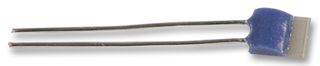
\includegraphics[width=0.5\textwidth]{DM-301.jpg}
	\caption{Foto do sensor resistivo Pt100, modelo DM-301, da LABFACILITY.}
	Fonte: \url{https://www.digchip.com/datasheets/parts/datasheet/2403/DM-301.php}
	\label{fig:DM-301}
\end{figure}

\begin{figure}[H]
	\centering 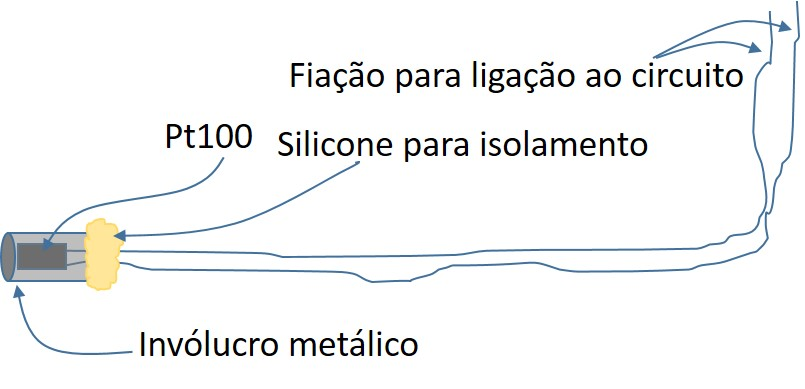
\includegraphics[width=0.5\textwidth]{termometro-ilustracao2.jpg}
	\caption{Ilustração com a montagem do sensor Pt100 em uma estrutura para utilização no experimento.}

	\label{fig:termometro-ilustracao}
\end{figure}

A classe B de tolerância, segundo a norma IEC751, apresenta um coeficiente térmico $\alpha = 0.003850 \Omega/\OmegaºC \pm 0.000063$, e um $R_0= 100\Omega \pm 0.12\%$. Os desvios admissíveis, para temperatura e resistência, são observados nas Equações \ref{eq:pt100-desvio-admissivel-temp} e \ref{eq:pt100-desvio-admissivel-resist}, respectivamente.

\begin{equation}
	T(ºC)=\pm (0.3+0.005*t)
	\label{eq:pt100-desvio-admissivel-temp}
\end{equation}
\begin{equation}
	R(\Omega)=\pm (0.12+0.0018*t)
	\label{eq:pt100-desvio-admissivel-resist}
\end{equation}

Usando-se os valores-padrão estabelecidos pela norma IEC751 para sensores Pt100, pode-se chegar à função de transferência teórica aproximada para esse sensor:

\begin{equation}
	R=R_0(1+\alpha(T-T_0))
	\label{eq:pt100-eq-teorica}
\end{equation}

\noindent onde $R_0$ é a resistência elétrica na temperatura $T_0$ e $\alpha$ é o coeficiente térmico da platina. Substituindo-se os valores na Equação \ref{eq:pt100-eq-teorica}, tem-se:

\begin{equation}
	R=100+0.385*T
	\label{eq:pt100-eq-teorica-valor}
\end{equation}

Sendo a sensibilidade teórica desse sistema representado por:

\begin{equation}
	S=0.385 [\Omega/ºC]
	\label{eq:pt100-sensibilidade-teorica-valor}
\end{equation}

Um típico condicionamento dado a RTDs utiliza o método baseado em uma ponte de Wheatstone. A Figura \ref{fig:termometro-ponte} apresenta o esquemático da estrutura básica da Ponte utilizada.

\begin{figure}[H]
	\centering 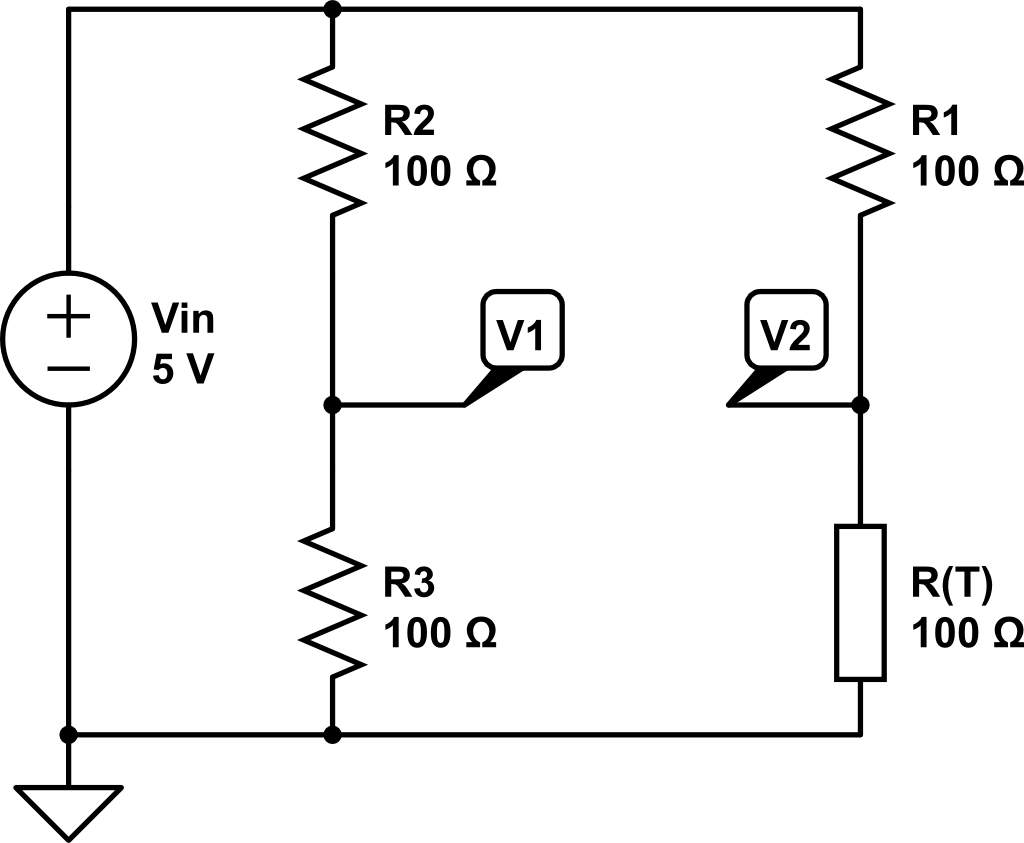
\includegraphics[width=0.5\textwidth]{pt100-ponte.png}
	\caption{Esquemático da estrutura básica da ponte de Wheatstone utilizada como parte do circuito condicionador do Pt100.}
	\label{fig:termometro-ponte}
\end{figure}

\noindent onde $R_1=R_2=R_3$ são resistores de $100\Omega\pm5\%$  e $R(T)$ é o sensor Pt100 com $100\Omega@0ºC$. $V_{in}$ é uma fonte de tensão de $5V$, e $V_1$ e $V_2$ são os nós diferenciais da ponte.

Equacionando o circuito apresentado na Figura \ref{fig:termometro-ponte}, para a saída diferencial, tem-se:

\begin{equation}
	V_{out}=V_1-V_2=\frac{R_2R(T)-R_3R_1}{(R_2+R_3)(R_1R(T))}V_{in}
	\label{eq:termometro-ponte-saida}
\end{equation}

Substituindo-se, na Equação \ref{eq:termometro-ponte-saida}, pelos valores nominais dos resistores e da fonte de alimentação, tem-se:

\begin{equation}
	V_{out}=2.5-\frac{500}{R(T)+100}
	\label{eq:termometro-ponte-saida-valores}
\end{equation}

A ponte de Wheatstone tem como característica principal de atingir tensão diferencial igual a zero para a seguinte relação de resistências elétricas:

 \begin{equation}
	R_1*R_3=R_2*R(T)
	\label{eq:termometro-ponte-equilibrio}
\end{equation}

Para os valores indicados, a situação explicitada na Equação \ref{eq:termometro-ponte-equilibrio} só acontece para $R(T)=100\Omega$, isto é, quando o sensor estiver percebendo uma temperatura de $0ºC$. Neste caso, a tensão diferencial é de $0V$.

Porém, como a temperatura mínima a ser medida é de $-10ºC$, é interessante que se tenha um circuito para o ajuste de balanço da ponte, na qual se consiga ajustar o valor de   saída em $0V$, independente do valor de $R(T)$. Para isso, foi adicionado um potenciômetro em paralelo com a ponte, com o cursor do potenciômetro ligado ao nó $V_2$ da ponte, conforme pode ser verificado na Figura \ref{fig:termometro-ponte-balanco}.

\begin{figure}[H]
	\centering 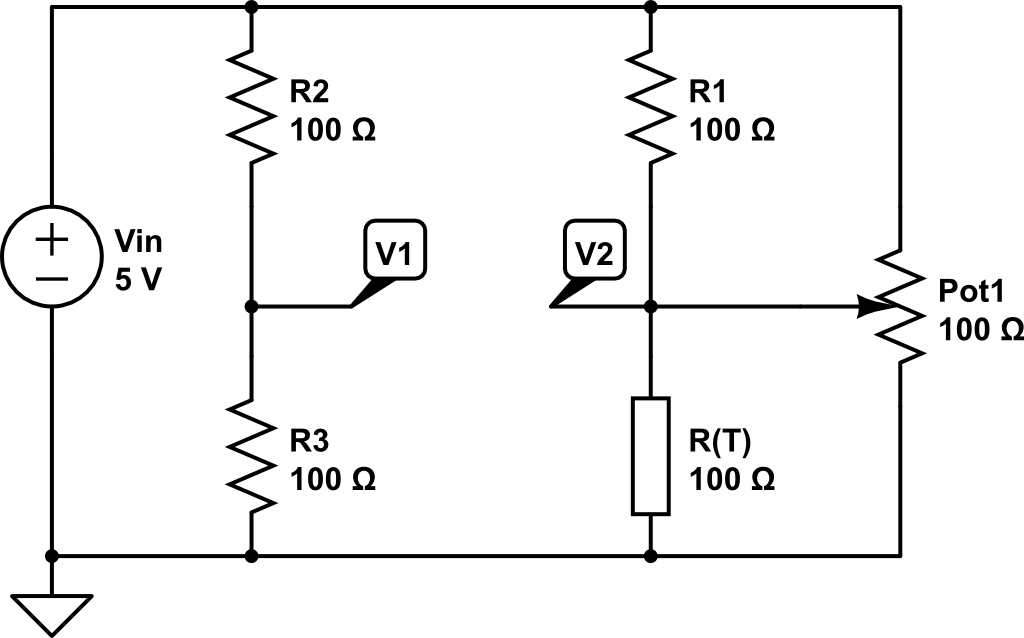
\includegraphics[width=0.7\textwidth]{pt100-ponte-balanco.png}
	\caption{Esquemático da estrutura básica da ponte de Wheatstone e um circuito para ajuste de balanço da ponte utilizada como parte do circuito condicionador do Pt100.}
	\label{fig:termometro-ponte-balanco}
\end{figure}

Associado ao circuito da ponte de Wheatstone com ajuste de balanço deve-se utilizar um amplificador de instrumentação (AI), a fim de deixar os níveis de tensão de saída mais apropriados ao nível de tensão de entrada do ADC. Para isto, foi utilizado o AI INA126 \cite{datasheet-INA126}, da Texas Instruments. Esse AI possui um ganho expresso por:

 \begin{equation}
	G=5+\frac{80k\Omega}{R_G}
	\label{eq:ganho-INA126}
\end{equation}

\noindent onde $R_G$ é um resistor conectado aos pinos 1 e 8 do CI, em função do ganho escolhido. Para o circuito implementado, foi utilizado um resistor de $100\Omega\pm5\%$ que, de acordo com a Equação \ref{eq:ganho-INA126}, obtém-se um ganho de, aproximadamente, 805 vezes.

Para controle de \textit{offset} da tensão de saída do AI foi adicionado ainda um \textit{trimpot} multivoltas de $10k\Omega$ alimentado com $+Vcc$ e $-Vcc$, e um resistor de $4.7k\Omega\pm5\%$ ligado ao nó $V1$ da ponte. Foi adicionado ainda um resistor de $1k\Omega\pm5\%$ em série com a alimentação e a ponte, a fim de limitar a corrente no circuito.

A Figura \ref{fig:termometro-ckt-condicionador-completo} mostra o circuito condicionador proposto para o Pt100, com a ponte de Wheatstone com ajuste de balanço, o circuito corretor de offset e o AI INA126.

\begin{figure}[H]
	\centering 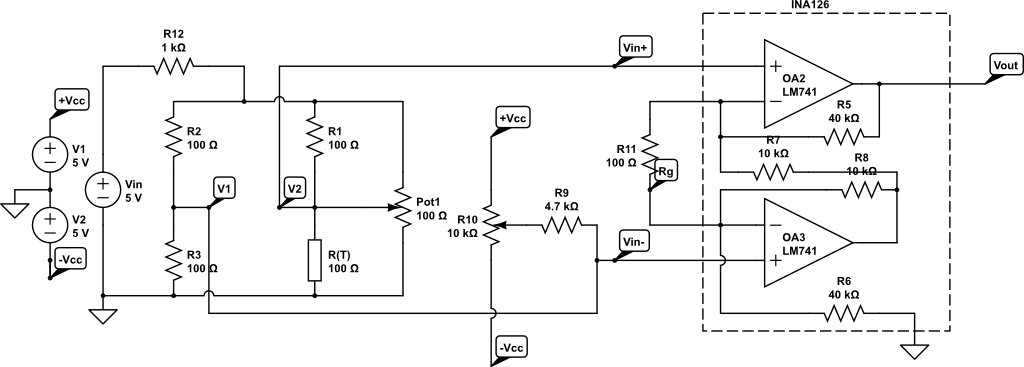
\includegraphics[width=\textwidth]{pt100-condicionamento-completo.png}
	\caption{Esquemático da estrutura básica de condicionamento proposto para o Pt100.}
	\label{fig:termometro-ckt-condicionador-completo}
\end{figure}

Com base na estrutura de condicionamento proposta e os valores teóricos da função de transferência do Pt100 (Equação \ref{eq:pt100-eq-teorica-valor}), pode-se elaborar a Cadeia de Medidas experimental proposta para o termômetro a ser implementado, verificada na Figura \ref{fig:termometro-cadeia-medidas-proposta}. Os potenciômetros de balanço e de \textit{offset} foram ajustados para uma saída próximo de $0V$ para uma temperatura de 20$ºC$, que é a metade do \textit{range} escolhido, representado por cerca de $108\Omega$.

\begin{figure}[H]
	\centering 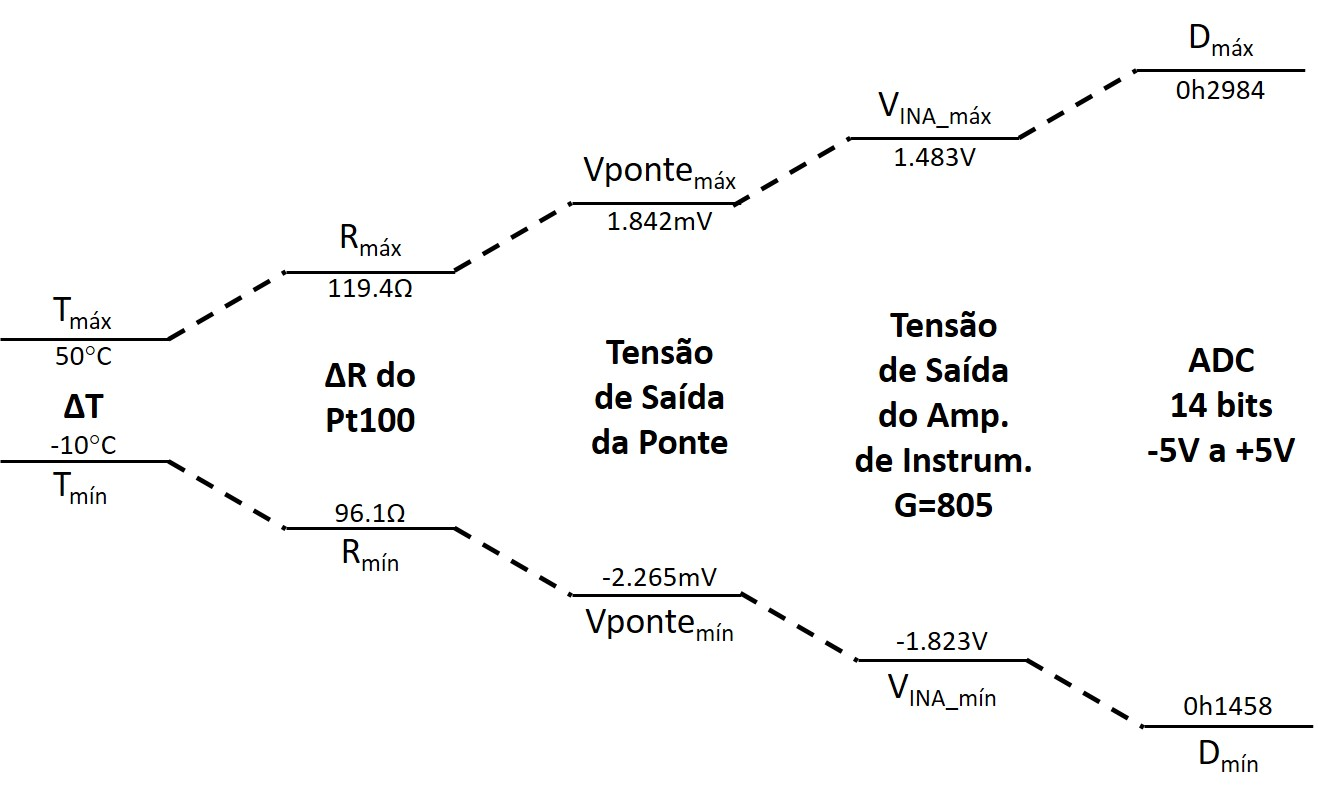
\includegraphics[width=\textwidth]{termometro-cadeia-medidas-proposta2.jpg}
	\caption{Cadeia de Medidas proposta para o termômetro a ser implementado.}
	\label{fig:termometro-cadeia-medidas-proposta}
\end{figure}

A Tabela \ref{tab:pt100-simulacao-ckt-condicionador} mostra os resultados de uma simulação feita com o circuito condicionador apresentado na Figura \ref{fig:termometro-ckt-condicionador-completo}, na qual foi modificado o valor do resistor R(T) de acordo com a função de tranferência teórica, variando a temperatura de $-10ºC$ a $+50ºC$, e observando-se a saída $V_{out}$, que é a saída do AI INA126.

\begin{table}[H]
\centering
\caption{Valores de simulação feita no circuito condicionado do Pt100, com variação de $-10ºC$ a $+50ºC$, observando-se a saída $V_{out}$ do circuito.}
\label{tab:pt100-simulacao-ckt-condicionador}
\begin{tabular}{|c|c|c|}
\hline
\textbf{$T (ºC)$} & \textbf{$R(T)(\Omega)$} & \textbf{$V_{out} (V)$} \\ \hline
-10             & 96.15         & -1.815              \\ \hline
-5              & 98.08         & -1.498              \\ \hline
0               & 100.00        & -1.193              \\ \hline
5               & 101.93        & -0.893              \\ \hline
10              & 103.85        & -0.604              \\ \hline
15              & 105.78        & -0.321              \\ \hline
20              & 107.70        & -0.046              \\ \hline
25              & 109.63        & 0.223               \\ \hline
30              & 111.55        & 0.483               \\ \hline
35              & 113.48        & 0.738               \\ \hline
40              & 115.40        & 0.986               \\ \hline
45              & 117.33        & 1.229               \\ \hline
50              & 119.25        & 1.465               \\ \hline
\end{tabular}
\end{table}

Realizando uma regressão linear entre as temperaturas e a tensão de saída do circuito, chega-se a uma função de transferência teórica/simulada do sistema, conforme a Equação \ref{eq:termometro-ft-simulada}

\begin{equation}
	V(T)=0.0546*T-1.1869 [V]
	\label{eq:termometro-ft-simulada}
\end{equation}

Que apresenta a seguinte sensibilidade:

\begin{equation}
	V(T)=54.6 [\frac{mV}{ºC}]
	\label{eq:termometro-sensibilidade-ft-simulada}
\end{equation}

A variação de $+0.1ºC$ na função de transferência teórica para o Pt100 dá uma variação de $+0.04\Omega$. Essa variação aplicada no circuito condicionador, de forma simulada, apresenta uma variação de $+7mV$ na saída do circuito. Com a configuração do ADC de 14bits, com entrada de $-5V$ a $+5V$, tem-se uma resolução de entrada de $0.61mV/bit$. Com isso, espera-se conseguir uma resolução teórica de $0.1ºC$ para entrada.

\section{Anemômetro}

O anemômetro é um instrumento que mede a velocidade do vento horizontal. Os anemômetros de copo são o tipo padrão de anemômetro, pois são robustos e resistentes aos ventos oblíquos causados por mastros e travessas, e este tipo foi utilizado neste projeto.

O experimento foi construído utilizando um modelo de anemômetro de copo com quatro hastes. Seu eixo e suas hastes foram feitas de madeira balsa, por apresentar baixa densidade e alta resistência. A ligação do eixo com a base foi feita por meio de um rolamento metálico de uso automotivo. Paralelo ao eixo, foi fixado um mastro para a colocação do sensor e, no eixo foi fixado um ímã de terras raras.

Como forma de medir a velocidade de rotação do anemômetro, foi utilizado um sensor de efeito \textit{Hall} associado com um ímã, conforme ilustra a Figura \ref{fig:anemometro-ilustracao}. Assim, toda vez que o ímã passar pelo sensor de efeito \textit{Hall}, este altera a sua tensão de saída, podendo assim ser contabilizado o número de voltas em um determinado período de análise.

\begin{figure}[H]
	\centering 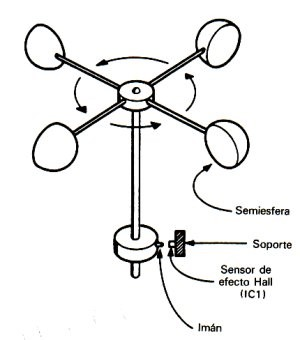
\includegraphics[width=0.5\textwidth]{anemometro-ilustracao.jpg}
	\caption{Ilustração de modelo de anemômetro a ser confeccionado.}
	Fonte:  \url{https://www.google.com.br/url?sa=i&rct=j&q=&esrc=s&source=images&cd=&ved=0ahUKEwje97Oi9pPNAhUMLyYKHTUiAOEQjBwIBA&url=http\%3A\%2F\%2Fs3.amazonaws.com\%2Fmagoo\%2FABAAAfwekAI-10.jpg&psig=AFQjCNFkGa7fc_vFBE0k5IBXnofWPzO8kQ&ust=1465320453086124}
	\label{fig:anemometro-ilustracao}
\end{figure}

O sensor utilizado no projeto foi o modelo SS94A2 \cite{datasheet-hall}, da Honeywell. A Figura \ref{fig:anemometro-hall-foto} apresenta a foto do sensor.

\begin{figure}[H]
	\centering 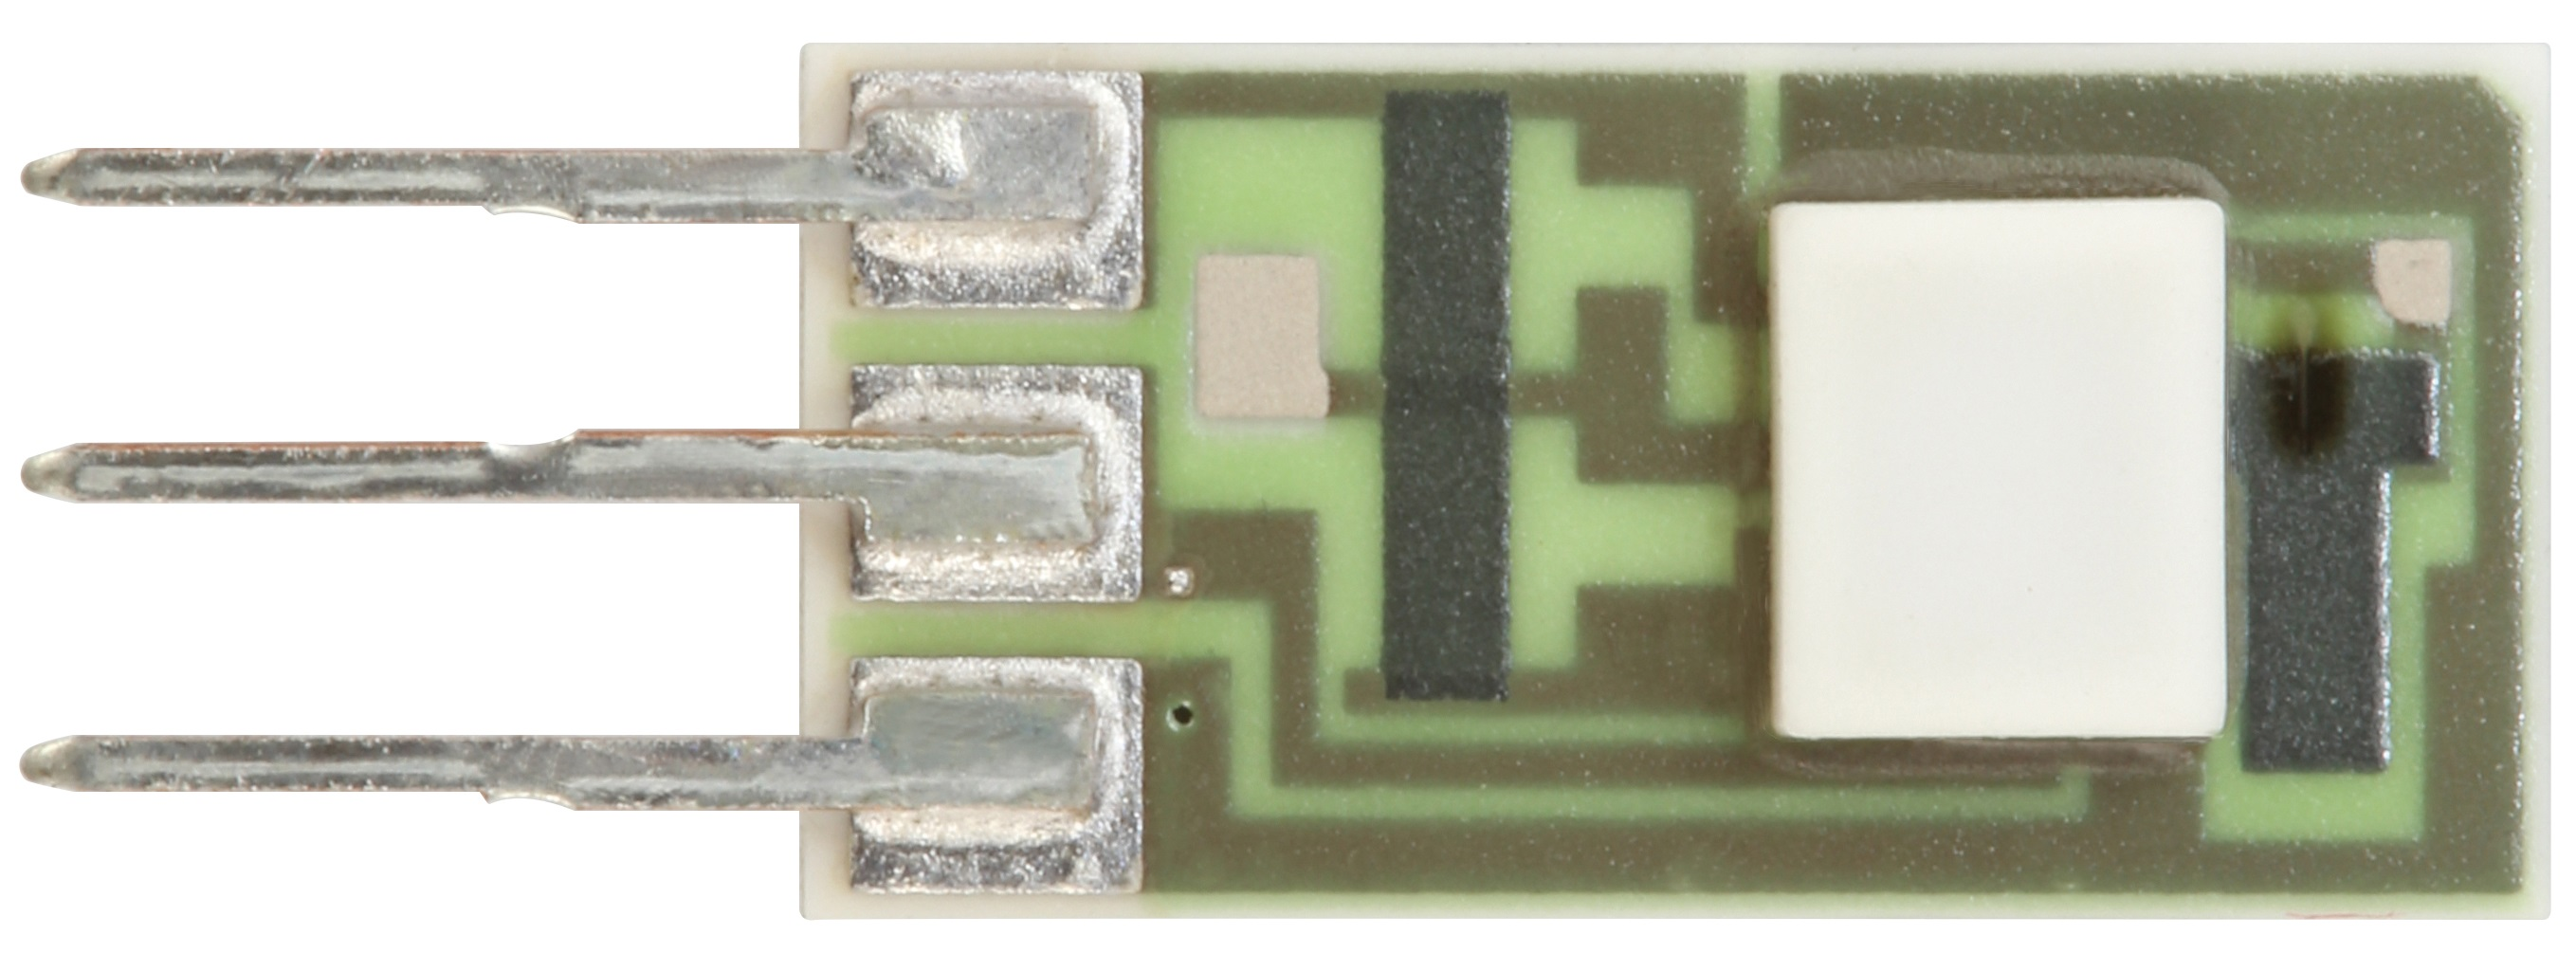
\includegraphics[width=0.5\textwidth]{sensor-hall-foto.jpg}
	\caption{Foto do sensor Hall modelo SS94A2, da Honeywell, utilizado na montagem experimental do anemômetro.}
	Fonte:  \url{http://sensing.honeywell.com/ss94a2-highres-photo.jpg}
	\label{fig:anemometro-hall-foto}
\end{figure}.

Na Figura \ref{fig:anemometro-bloco-experimental} verifica-se o digrama de blocos proposto para para a implementação experimental do anemômetro.

\begin{figure}[H]
	\centering 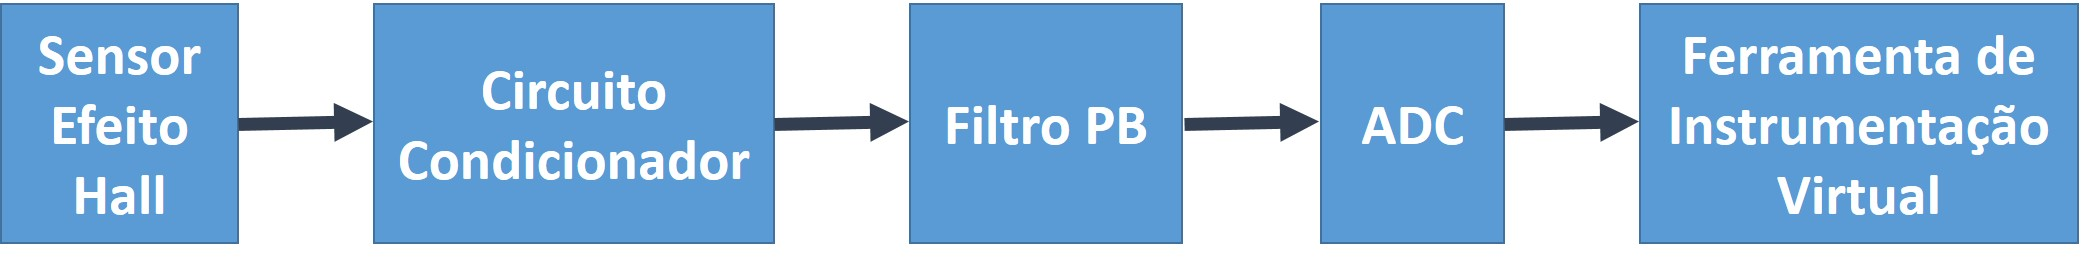
\includegraphics[width=0.8\textwidth]{anemometro-fluxograma.jpg}
	\caption{Diagrama de blocos proposto para implementação experimental do anemômetro.}
	\label{fig:anemometro-bloco-experimental}
\end{figure}.

O sensor Hall utilizado possui três terminais, dos quais 2 deles são para alimentação, e o terceiro é a saída do sensor. De acordo com o datasheet do fabricante \cite{datasheet-hall}, quando na ausência de magnetismo, a saída do sensor permanece em um valor constante de 4.00$V$ $\pm$ 0.04$V$ a 25$ºC$. Com a aproximação de um campo magnético positivo, sua tensão aumenta em 5.0$mV$ $\pm$ 0.1$mV$ por \textit{gauss}, que é a unidade de densidade de fluxo magnético. Se o campo for negativo, a tensão diminui nas mesmas proporções.

Como a intenção do uso do sensor é apenas para a contagem da rotação da estrutura do anemômetro, não interessa a intensidade do fluxo magnético em si, mas apenas a sua presença ou não. Isto é, com a presença de um campo magnético positivo, a tensão no terminal de saída do sensor sobe e assim é possível executar a contagem dos giros.

Para facilitar essa contagem, foi montado um circuito condicionador que discretiza o sinal por meio de um circuito \textit{Schmitt Trigger}, isto é, quando o sinal cruza por um certo valor de tensão, a saída do sistema se altera de 0$V$ para $+Vcc$, provocando um chaveamento no sinal de saída. Com isso, tem-se na saída do circuito uma onda quadrada. O circuito apresentado na Figura \ref{fig:hall-circuito} foi implementado para executar a função de chaveamento do sinal. 

\begin{figure}[H]
	\centering 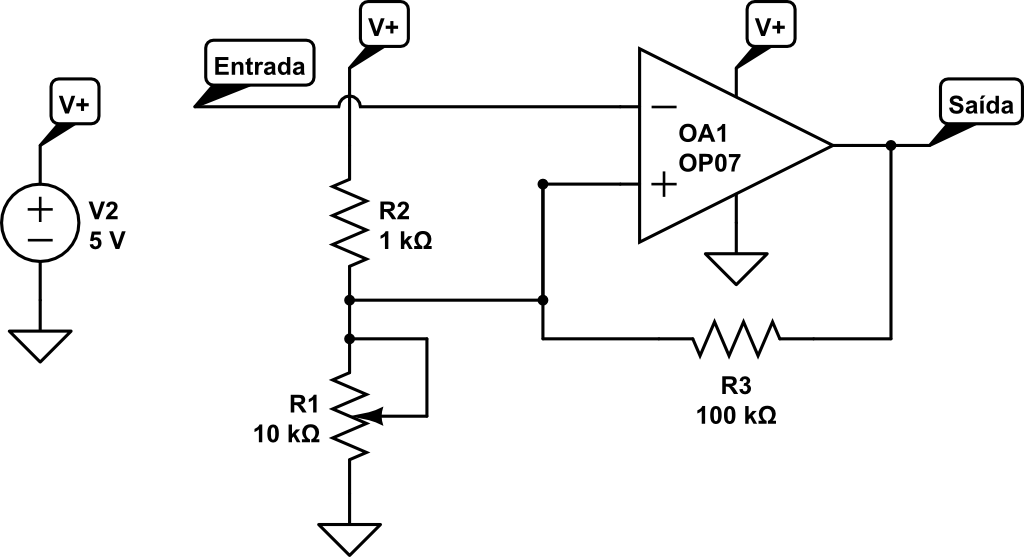
\includegraphics[width=0.7\textwidth]{hall-circuito.png}
	\caption{Esquemático básico do sistema de condicionamento de chaveamento do sensor Hall.}
	\label{fig:hall-circuito}
\end{figure}.

Foi utilizado um potenciômetro para poder realizar o ajuste da tensão limite para a realização do chaveamento. Por se tratar de um circuito comparador inversor, quando a tensão de entrada está abaixo do limite estipulado, a saída permanece em $+Vcc$. Quando a entrada passa para valores acima do estipulado, a saída vai para 0$V$, votando para $+Vcc$ quando a tensão de entrada cair para valores abaixo do ajustado.

Foi estipulada uma faixa de trabalho de 3$m/s$ a 15$m/s$, com uma resolução de saída de 0.1$m/s$. Para a determinação da velocidade do vento verificou-se a quantidade de RPM (rotações por minuto) e calculou-se a velocidade tangencial na extremidade das hastes do anemômetro, utilizando-se a Equação \ref{eq:anemometro-rpm-to-vtan}.

\begin{equation}
	v=\frac{\mathrm{RPM}*2*\pi*r}{60}[m/s]
	\label{eq:anemometro-rpm-to-vtan}
\end{equation}

\noindent onde $v$ é a velocidade tangencial na extremidade das hastes e $r$ é o comprimento de cada haste, em metros.

Para uma estrutura com hastes de 18cm, como foi utilizado no projeto experimental, para os limites inferior e superior da faixa de trabalho estipulada, tem-se 159 RPM e 796 RPM, respectivamente, representando 2.65$Hz$ e 13.27$Hz$. A Equação \ref{eq:anemometro-FT-proposta} explicita a função de transferência do sistema, com a velocidade do vento, dada em $m/s$, em função da rotação das hastes, dada em RPM.

\begin{equation}
	v=0.01885*\mathrm{RPM} [m/s]
	\label{eq:anemometro-FT-proposta}
\end{equation}

\noindent que apresenta uma sensibilidade de:

\begin{equation}
	S=0.01885 \left [ \frac{m/s}{\mathrm{RPM}} \right ]
	\label{eq:anemometro-sensibilidade-proposta}
\end{equation}

A Figura \ref{fig:anemometro-cadeia-medidas-proposta} apresenta a cadeia de medidas proposta, tomando por base os limites estipulados.

\begin{figure}[H]
	\centering 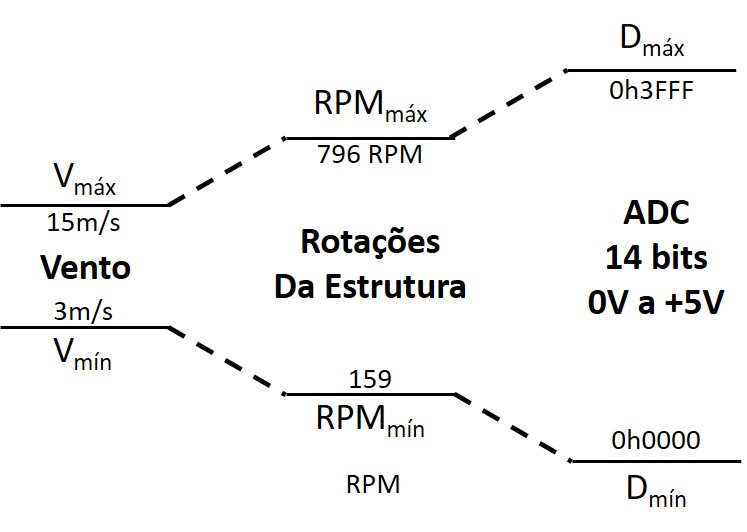
\includegraphics[width=0.5\textwidth]{anemometro-cadeia-medidas-proposta.jpg}
	\caption{Cadeia de medidas proposta para o anemômetro a ser implementado.}
	\label{fig:anemometro-cadeia-medidas-proposta}
\end{figure}.

Haja vista que a velocidade medida é a velocidade de giro dos braços do anemômetro, é de se esperar que este valor não condiza exatamente com o valor do vento que faz girar a estrutura, já que o sistema apresenta um arrasto agindo contra a força que o vento exerce sobre a estrutura. Assim, para se ter o valor correto de velocidade do vento, um anemômetro digital modelo LM-8010 \cite{anemometro-manual}, da Lutron Electronic, que na escala de $m/s$ trabalha em um range de 0.4 a 30.0$m/s$, com uma resolução de 0.1$m/s$, e uma precisão de $\pm$ 3$\%$ do fundo de escala para medidas até 20$m/s$ e de $\pm$ 4$\%$ do fundo de escala para medidas acima de 20$m/s$, foi utilizado para se realizar a comparação com o vento aplicado no equipamento experimental e a saída apresentada, a fim de se obter sua função de transferência.

No Labview foi criado um \textit{script} que faz a leitura da saída do circuito condicionador, que presenta uma onda quadrada quando a estrutura experimental está girando. Desta forma, é possível calcular o período de cada volta, utilizando um bloco de \textit{MATLAB Script} que conta o tempo entre as bordas de descida da onda, fornecendo assim o período de oscilação.

\section{Pluviômetro}
O pluviômetro é um aparelho de meteorologia usado para recolher e medir, em milímetros lineares, a quantidade de líquidos ou sólidos (chuva, neve, granizo) precipitados durante um determinado tempo e local. O parâmetro determinado por esse instrumento chama-se \textit{índice pluviométrico}, que é o somatório da precipitação num determinado local durante um período de tempo estabelecido, medido em milímetros [$mm$]. Como o equipamento mensura a quantidade de chuva que precipita, em conjunto com o sensor de temperatura, são variáveis elementares para estudos meteorológicos e hidrológicos.

A estrutura física do pluviômetro consiste em um sistema de captação de chuva, com uma área determinada, e um reservatório para coleta do material captado. Nesse reservatório há um sensor que possibilita medir a diferença do nível de fluído armazenado, calculando assim o índice pluviométrico em milímetros, que indica o volume em litros de água que caíram em um metro quadrado de área, assim uma chuva de 20 mm corresponderá à precipitação de 20 litros de água por metro quadrado, logicamente sempre na horizontal. Como quaisquer equipamentos automáticos, um \textit{software} de coleta e tratamento de dados é utilizado para relatórios temporais e análises das características da chuva.

Para cálculo do índice pluviométrico (ou pluviosidade), dado em mm, é a relação do volume de água recolhida, em litros, pela área de abertura do coletor de precipitação, em $m^2$. Para facilitação dos cálculos, partiu-se do princípio que o coletor compõe-se de um funil com um dimâmetro de entrada de 13.82$cm$, conforme ilustra a Figura \ref{fig:pluviometro-funil}. Parte-se do princípio que a chuva caiu na vertical e que toda a água coletada na entrada do funil foi para o reservatório, não havendo assim perdas.

\begin{figure}[H]
	\centering 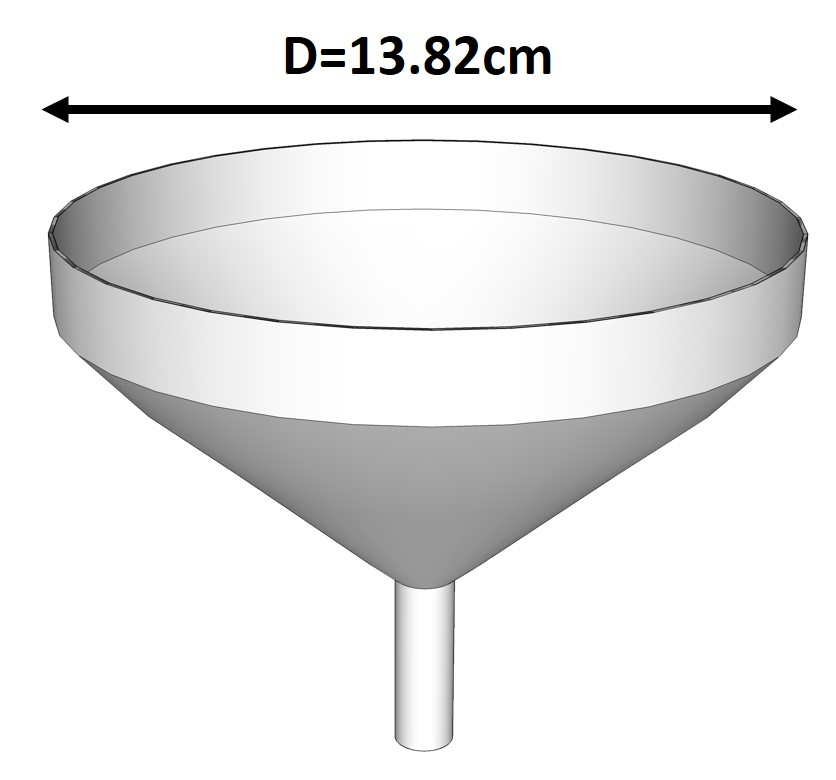
\includegraphics[width=0.5\textwidth]{pluviometro_funil.jpg}
	\caption{Ilustração com dimensão de entrada do funil coletor do pluviômetro.}
	\label{fig:pluviometro-funil}
\end{figure}

Com esse diâmetro é possível calcular a área de coleta, conforme a Equação \ref{eq:pluviometro-indice-area}.

\begin{equation}
	A=\pi*r^2=\pi*\left ( \frac{D}{2} \right )^2=\pi*\left ( \frac{0.1382m}{2} \right )^2=0.015m^2
	\label{eq:pluviometro-indice-area}
\end{equation}

Como a pluviosidade é dada pelo volume coletado divido pela área de coleta, dada a área, tem-se que, a cada 1.5$mL$ coletado, equivale a 1$mm$ de chuva, ou seja, é como se tivesse chovido 1$L$ em 1$m^2$. Assim, determinou-se a resolução de saída do sistema em 1$mm$.

Optou-se por utilizar um sensor capacitivo com referência baseada em um documento do "TI Designs"\cite{pluviometro-capacitivo-texas} onde é proposto um sensor simples de medida de capacitância utilizando uma placa de circuito impresso com duas placas paralelas co-planares. A fim de determinar a validade do \textit{design} de sensor, foi confeccionado um sistema simples com uma placa de circuito impresso contendo duas barras que funcionam como eletrodos do sensor e a placa foi fixada na face interna de um recipiente de acrílico. A placa foi isolada com verniz e papel \textit{contact} para evitar que a água fizesse contato elétrico entre os eletrodos. O recipiente possui dimensões internas de 3cm por 6cm com 15cm de altura e foi confeccionado sob medida.

A Figura \ref{fig:sensor-nivel-capacitivo} apresenta um desenho esquemático do sensor de nível

\begin{figure}[H]
	\centering 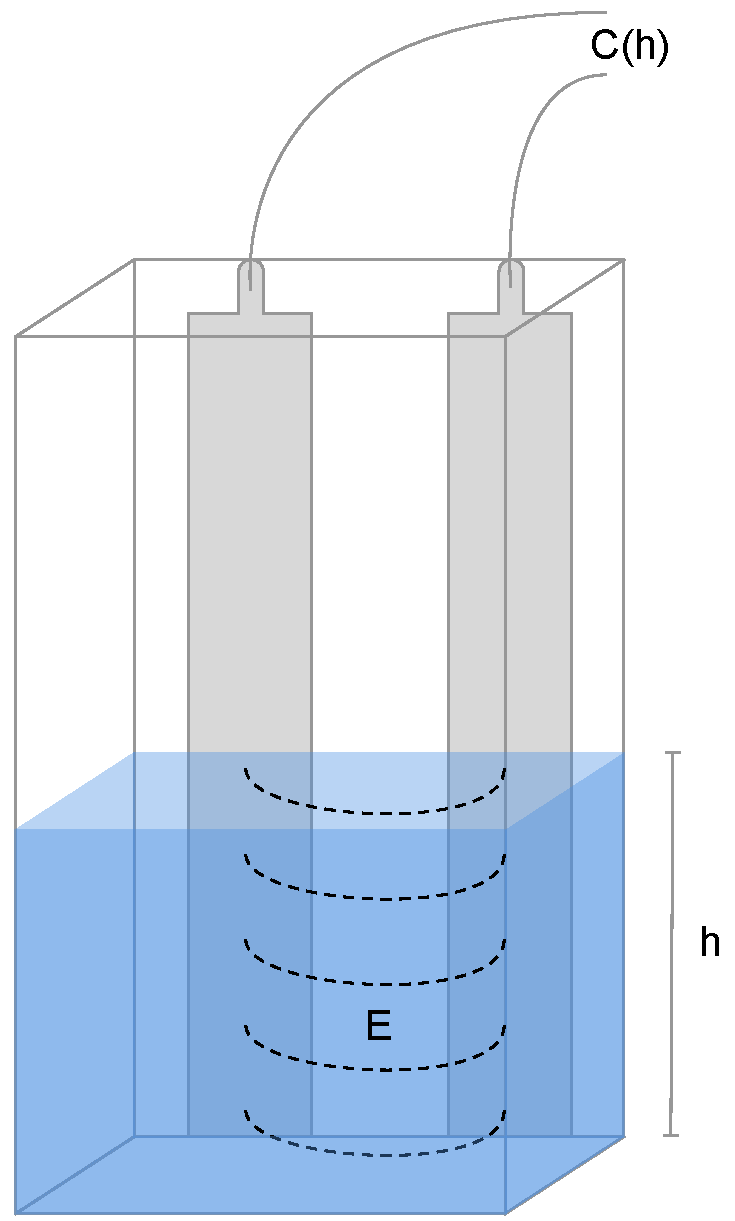
\includegraphics[width=0.5\textwidth]{SensorNivelCapacitivo.pdf}
	\caption{Desenho esquemático do sensor de nível capacitivo. $C(H)$ é a capacitância equivalente da construção para um nível de água $h$ e $E$ são as linhas de campo elétrico internas no sensor.}
	\label{fig:sensor-nivel-capacitivo}
\end{figure}

A fim de determinar a viabilidade de medição deste sistema, um experimento rápido foi realizado onde a função de transferência da capacitância do sistema foi extraída utilizando uma ponte LCR comercial Minipa MX-1010 \cite{ponte-minipa} em modo série com frequência de 1 kHz para a medição da capacitância para volumes de água entre 0 mL e 118 mL com resolução de 1mL.

Com o intuito de estimar o valor de capacitância do sistema, foi utilizado um circuito de condicionamento misto digital e analógico. Na parte analógica, um oscilador controlado pela capacitância do sensor foi utilizado. O oscilador gera uma onda quadrada com frequência (e período) variável que depende diretamente do valor de capacitância do sensor. A Figura \ref{fig:metodologia-capacitivo-oscilador} apresenta o esquemático do oscilador.

\begin{figure}[H]
	\centering
	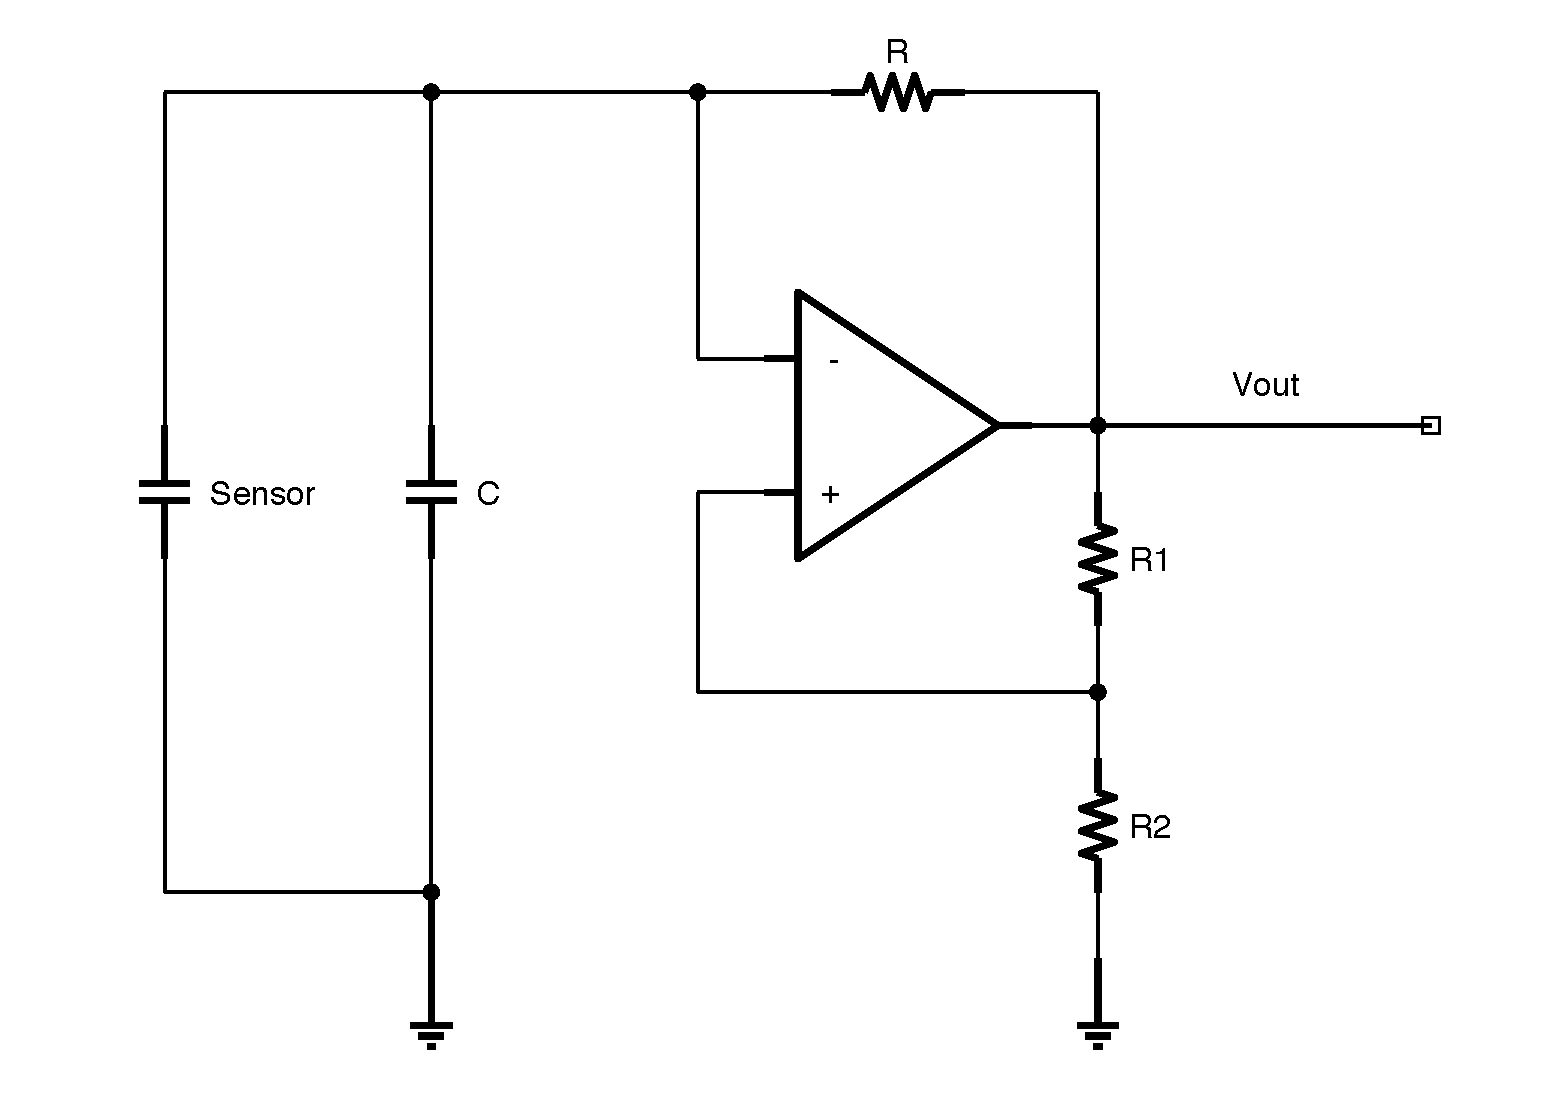
\includegraphics[width=0.7\textwidth]{Circuitos/Pluviometro-Oscilador.pdf}
	\caption{Esquemático do oscilador utilizado no circuito de condicionamento do sensor de nível capacitivo}
	\label{fig:metodologia-capacitivo-oscilador}
\end{figure}

Neste sistema, a equação teórica que determina o período de oscilação do sistema é dada pela expressão da Equação \ref{eq:metologia-pluviometro-periodo}.

\begin{equation}
	T = 2 R C ln \left(\frac{1+\lambda}{1-\lambda}\right)
	\label{eq:metologia-pluviometro-periodo}
\end{equation}
\noindent onde $R$ é o resistor de realimentação positiva, C é o valor de capacitância do oscilador, $ln$ é o logaritmo natural neperiano e $\lambda$ é definido conforme a expressão da Equação \ref{eq:metologia-pluviometro-periodo-2}.

\begin{equation}
	\lambda = \frac{R_1}{R_1 + R_2}
	\label{eq:metologia-pluviometro-periodo-2}
\end{equation}
\noindent onde $R_1$ e $R_2$ consiste nos resistores de realimentação positiva do circuito.

Para evitar que a frequência ficasse num valor muito alto, ou seja, períodos muito baixos, o que torna mais dificultosa a medida, foi adicionado um capacitor de $40 nF$ em paralelo com o sensor cuja única função é limitar a frequência de oscilação do sistema.

No sistema montado foram utilizados os seguintes componentes indicados nas Equações \ref{eq:metodologia-pluviometro-componentes}

\begin{eqnarray}
	R &=& (2.2 M\Omega \pm 10\%) 		\label{eq:metodologia-pluviometro-componentes}					\\
	C &=& (27 pF \pm 20\%) + C(V) 		\nonumber			\\
	R_1 = R_2 &=& (10 k\Omega \pm 10\%)	\nonumber
\end{eqnarray}
\noindent onde $C(V)$ é o valor de capacitância do sensor correspondente ao volume $V$ em $mL$.

Como amplificador operacional para o oscilador foi utilizado um OP27 fabricado pela \textit{Analog Devices} com resistências típicas de entrada diferencial de $6 M\Omega$ e modo comum de $3 G\Omega$. Estes valores são significativoss perante o valor de resistência elétrica utilizado na realimentação do negativa do circuito.

Em termos práticos, foi utilizado um sistema com três entradas para que haja compensação da variação de temperatura ambiente, ou seja, o líquido deve estar à mesma temperatura ambiente do sensor de referência externa. A expressão da Equação \ref{eq:metodologia-pluviometro-compensacao} apresenta a expressão utilizada para agregar os valores dos 3 sensores num único valor.

\begin{equation}
	N = \frac{C(V) - C(0)}{C_{ref} - C_{ambiente}}
	\label{eq:metodologia-pluviometro-compensacao}
\end{equation}
\noindent onde $N$ é uma unidade adimensional sem significado físico que atribui um valor numérico ao sistema de medida, $C(V)$ é o valor correspondente de capacitância do sensor para um volume $V$, $C(0)$ é o valor de capacitância do sistema quando sem líquido (à vazio), $C_{ref}$ é o valor de capacitância do sensor de referência de líquido e $C_{ambiente}$ é o sensor externo que compensa variações externas de temperatura.

A expressão teórica da capacitância pode ser aproximada utilizando as expressões propostas por Lawrenson em \textit{Analysis and Computation of Electric and Magnetic Field Problems}\cite{capacitor-plano} em 1973, conforme a Equação \ref{eq:metodologia-pluviometro-capacitancia-coplanar}:

\begin{equation}
	C_{cp} = \epsilon l \frac{K\left(\sqrt{1-\frac{d^2}{4 (d+w_1) (d+w_2)}}\right)}{K\left(\frac{1}{2} \sqrt{\frac{d^2}{(d+w_1) (d+w_2)}}\right)}
	\label{eq:metodologia-pluviometro-capacitancia-coplanar}
\end{equation}
\noindent onde $C_{cp}$ é a capacitância de um capacitor com duas placas co-planares, $K(x)$ é a integral elíptica do primeiro tipo, $\epsilon$ é a permissividade elétrica do dielétrico, $l$ é o comprimento das faixas, $d$ é o espaçamento entre as placas co-planares e $w_1$ e $w_2$ são as larguras das placas do capacitor.

No caso específico do sensor de nível, é possível dividir este capacitor em 2 subcapacitores em paralelo: um cujo dielétrico é o ar e outro cujo dielétrico é a água. A expressão da Equação \ref{eq:metodologia-pluviometro-capacitancia-relacao} define a relação entre os capacitores de forma matemática.

\begin{equation}
	C(h) = C_{cp}\left(l=H-h, \epsilon=\epsilon_{ar}\right) + C_{cp}\left(l=h, \epsilon=\epsilon_{agua}\right)
	\label{eq:metodologia-pluviometro-capacitancia-relacao}
\end{equation}
\noindent onde $C(h)$ é a capacitância para um nível $h$ de água, $H$ é a altura total do sensor e $C_{cp}$ é a expressão da Equação \ref{eq:metodologia-pluviometro-capacitancia-coplanar}.

Substituindo as constantes físicas $\epsilon_{ar}$ e $\epsilon_{agua}$ na equação e simplificando, obtém-se a Equação \ref{eq:metodologia-pluviometro-capacitancia-teorico} que dá a função de transferência experimental do sistema para a capacitância do sensor em $pF$.

\begin{equation}
	C(h) = \frac{(700.035 h+8.85 H) K\left(\sqrt{1-\frac{d^4}{16 (d+w)^4}}\right)}{K\left(\frac{1}{2} \sqrt{\frac{d^2}{(d+w)^2}}\right)}
	\label{eq:metodologia-pluviometro-capacitancia-teorico}
\end{equation}
\noindent onde $C(h)$ é a capacitância do sensor para o nível de água $h$, $K(x)$ é a integral elíptica do primeiro tipo, $H$ é a altura do sensor, $d$ é o espaçamento entre as placas co-planares e $w$ é a largura das placas do capacitor.

A Equação \ref{eq:metodologia-pluviometro-capacitancia-teorico} não pode ser simplificada além pois não há solução simbólica para a integral elíptica dada. Uma solução final pode ser obtida substituindo as dimensões físicas do sensor utilizado. O sensor possui as características físicas dadas pelas Equações \ref{eq:metodologia-pluviometro-capacitancia-caracteristicas-1}, \ref{eq:metodologia-pluviometro-capacitancia-caracteristicas-2}, \ref{eq:metodologia-pluviometro-capacitancia-caracteristicas-3}.

\begin{eqnarray}
	H &=& 13.5cm \label{eq:metodologia-pluviometro-capacitancia-caracteristicas-1} \\
	w &=& 1.80cm \label{eq:metodologia-pluviometro-capacitancia-caracteristicas-2} \\
	d &=& 1.40cm \label{eq:metodologia-pluviometro-capacitancia-caracteristicas-3}
\end{eqnarray}

A Equação \ref{eq:metodologia-pluviometro-capacitancia-teorico-final} apresenta a função de transferência final após a substituição das características físicas do sensor.

\begin{equation}
	C(h) = 3.41655 + 2001.85 h
	\label{eq:metodologia-pluviometro-capacitancia-teorico-final}
\end{equation}
\noindent onde $C(h)$ é a capacitância (em pF) do sensor para uma coluna $h$ (em metros) de água.

Substituindo a coluna de água por volume (as calibrações foram realizadas em função do volume de água por facilitar as medições) na Equação \ref{eq:metodologia-pluviometro-capacitancia-teorico-final} o valor de capacitância é dado conforme Equação \ref{eq:metodologia-pluviometro-capacitancia-teorico-volume}

\begin{equation}
	C(V) = 3.41655 + 1.66821 V
	\label{eq:metodologia-pluviometro-capacitancia-teorico-volume}
\end{equation}
\noindent onde $C(V)$ é a capacitância (em pF) do sensor para um volume $V$ (em mL) de água dentro do recipiente.

A Figura \ref{fig:metodologia-pluviometro-teorico-capacitancia} apresenta de forma gráfica a função de transferência do sensor para o seu valor de capacitância.

\begin{figure}[H]
	\centering
	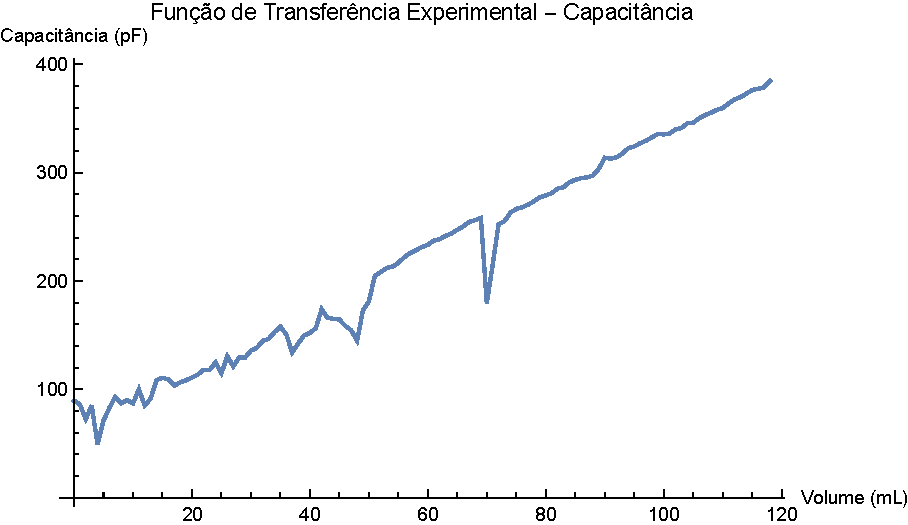
\includegraphics[width=\textwidth]{Nivel/Teorico/Capacitancia.pdf}
	\caption{Função de Transferência para o valor de capacitância do sensor}
	\label{fig:metodologia-pluviometro-teorico-capacitancia}
\end{figure}

Na Figura \ref{fig:metodologia-pluviometro-teorico-capacitancia} observa-se que a variação de capacitância em função do volume de água é linear. A sensibilidade do sistema é dada pela expressão da Equação \label{eq:metodologia-pluviometro-teorico-capacitancia-sensibilidade}

\begin{eqnarray}
	S &=& 1.66821 pF/mL \\
	  &=& 2.00185 pF/mm \nonumber
	\label{eq:metodologia-pluviometro-teorico-capacitancia-sensibilidade}
\end{eqnarray}
\noindent são as sensibilidades para o volume de líquido e para a coluna de líquido.

Observando-se a equação \ref{eq:metologia-pluviometro-periodo} é possível notar que, desde que os componentes passivos permaneçam constantes, a relação entre a capacitância e o período de oscilação é direta e dada pela multiplicação de uma constante, conforme mostrado na Equação \ref{eq:metologia-pluviometro-periodo-simplificado}.

\begin{equation}
	T = 2 R C ln \left(\frac{1+\lambda}{1-\lambda}\right) = k C
	\label{eq:metologia-pluviometro-periodo-simplificado}
\end{equation}
\noindent onde $T$ é o período de oscilação do oscilador, $C$ é a capacitância do sensor e $k$ é uma constante definida pelos componentes passivos do sistema.

Dessa forma, é possível considerar tanto o período quanto a capacitância para cálculo da grandeza $N$ (Equação \ref{eq:metodologia-pluviometro-compensacao}) do sistema. Portanto, a segunda parte do sistema é realizada digitalmente utilizando um microcontrolador MSP430G2553 da Texas Instruments onde um \textit{timer} de 16 bits à uma frequência de (16 $\pm$ 0.48) MHz foi utilizado para calcular o período da forma de onda gerada pelo oscilador.

O programa microcontrolado foi desenvolvido em C++ utilizando o compilador mspgcc (um \textit{port} do \textit{GNU C Compiler} para o MSP430) versão "msp430-gcc (MSPGCC 20120406 (With patches: sf3540953 sf3559978)) 4.6.3 20120301 (mspgcc LTS 20120406 unpatched)". Neste programa, um \textit{timer} de 16 bits de contagem contínua crescente foi iniciado à (16 $\pm$ 0.48) MHz. A cada \textit{overflow} do \textit{timer} um segundo contador e 64 bits era incrementado em 1. Desta forma, era possível obter um v efetivo de 80 bits mas por limitação técnica do processador os últimos 16 bits do segundo contador eram descartados, totalizando em 64 bits efetivos. Vale ressaltar que destes 64 bits, 16 deles eram acionados pelo \textit{timer} interno do processador e os 48 restantes gerados por \textit{software} usando interrupções do v. Este contador é denominado de "temporizador" no restante deste documento. Técnicas semelhantes a estas são utilizadas nos diversos sistemas operacionais de computador doméstico utilizados comercialmente hoje em dia.

\begin{lstlisting}[caption=Rotina de extração do timer do temporizador]
typedef uint64_t counter_t;
static counter_t counter_time() {
    // shifts the incrementing counter by 16 bits to the left
    // and appends the 16-bit timer to the result
    return TA0R | ((counter & 0x0000FFFF) << 16);
}
\end{lstlisting}

Na inicialização do processador três interrupções de borda de descida eram ativadas para cada um dos sensores e quando disparadas, o valor do temporizador era obtido e salvo na memória do processador. No próximo disparo de interrupção um novo valor do temporizador é extraído e a diferença entre o temporizador do ciclo anterior e do atual são subtraídos e este resultado determina o número $N$ de ciclos do processador entre as duas bordas de subida do sinal, isto é, indiretamente representa o período do oscilador.

Uma vez que o \textit{timer} está sendo incrementado à uma taxa de (16 $\pm$ 0.48) MHz, o tempo real de oscilação pode ser obtido pela relação da Equação \ref{eq:metodologia-pluviometro-relacao-ciclos-tempo}:

\begin{equation}
	T_{real} = \frac{16 000 000}{n_{ciclos}}
	\label{eq:metodologia-pluviometro-relacao-ciclos-tempo}
\end{equation}

A função de transferência teórica para o sistema é dada pela Equação \ref{eq:metodologia-pluviometro-ciclos-teorico}

\begin{eqnarray}
	n &=& 8768.36 + 480.903 V \text{ (ciclos)} \label{eq:metodologia-pluviometro-ciclos-teorico} \\
	  &=& 8768.36 + 577084 h \text{ (ciclos)} \nonumber
\end{eqnarray}
\noindent onde $n$ é o número de ciclos em uma oscilação, $V$ é o volume de água em mL dentro do recipiente e $h$ é a altura de líquido em metros dentro do recipiente.

A sensibilidade do sistema é dada pela Equação \ref{eq:metodologia-pluviometro-ciclos-teorico-sensibilidade}

\begin{eqnarray}
	S &=& 480.903 \text{ ciclos/mL} \label{eq:metodologia-pluviometro-ciclos-teorico-sensibilidade} \\
	  &=& 577.084 \text{ ciclos/mm} \nonumber
\end{eqnarray}

O valor de contagem de ciclos (e seu correspondente em tempo real) foram validados utilizando um osciloscópio Tektronix TDS2002C.

Para transferir os dados para um computador foi utilizado o controlador de serial por hardware do próprio processador para comunicar via UART com o computador. A placa desenvolvimento do MSP430 já possui adaptador UART-USB para conexão com o computador, esta mesma que impõe um limite da \textit{baud rate} de no máximo 9600 bps. Periodicamente o processador envia os dados pela comunicação serial utilizando um pacote de dados com a seguinte estrutura, expressa conforme uma estrutura em C:

\begin{lstlisting}[caption=Estrutura dos pacotes de conteúdo enviados pela linha de comunicação serial, language=C++, directivestyle={\color{black}} emph={int,char,double,float,unsigned,uint8_t}, emphstyle={\color{blue}}]
/**
 * The type used to represent a number of cycles
 */
typedef uint32_t cycles_t;

/**
 * A structure containing the measurement ID and cycle count
 */
struct measurement_t {
    /**
     * The measurement ID
     */
    uint8_t id;

    /**
     * The number of cycles that happened between the last two 
     * oscillator low borders
     */
    cycles_t cycleCount;
};

/**
 * The level sensor communication protocol packet structure
 */
struct packet_payload {
    /**
     * A sync packet that indicates the start of a sequence
     */
    uint8_t sync;

    /**
     * A measurement payload representing the level sensor
     */
    measurement_t level;

    /**
     * A measurement payload representing the reference sensor
     */
	measurement_t reference;

    /**
     * A measurement payload representing the environment sensor
     */
    measurement_t environment;
};
\end{lstlisting}

Periodicamente um pacote "packet\_payload" é enviado com os dados de todas as medidas. O campo "sync" possui um byte de sincronia fixo definido arbitrariamente com o valor hexadecimal de $0xFB$. O cliente, ao iniciar a comunicação aguarda até o recebimento do campo de sincronia e então começa a leitura dos dados de forma sequencial.

O programa completo se encontra no anexo \todo{anexo do msp430}.

No computador, foi implementado uma classe em C++11 utilizando APIs \textit{POSIX} (\textit{Portable Operating System Interface}, padrão definido pela IEEE para interoperabilidade de sistemas operacionais) para a leitura de dados da porta serial. A classe pode ser compilada e utilizada em qualquer sistema operacional \textit{UNIX-like} como Apple Mac OS X, Linux, FreeBSD ou Solaris. Esta classe apenas oferece uma forma assíncrona de acesso aos dados e não implementa nenhuma interface gráfica e automaticamente implementa um filtro passa-baixas digital para a suavização e remoção de ruído do sinal. A frequência de corte é de 1 Hz.

Para a interface gráfica utilizada para a interação homem-máquina, foi desenvolvido um aplicativo para Apple Mac OS X 10.11.5 utilizando a linguagem de programação Objective-C para as partes nativas do sistema (\textit{Cocoa}) e Objective-C++ para comunicação com o sistema de aquisição de dados via serial.

Por conter arquivos muito grandes para a inclusão em anexo, o código completo do programa se encontra em um repositório no GitHub na seguinte \textit{URL}:

\url{https://github.com/Rogiel/ufrgs-instrumentacao-projeto}

A Figura \ref{fig:pluviometro-cadeia-medidas-proposta} apresenta a cadeia de medidas proposta para o instrumento experimental do pluviômetro.

\begin{figure}[H]
	\centering
	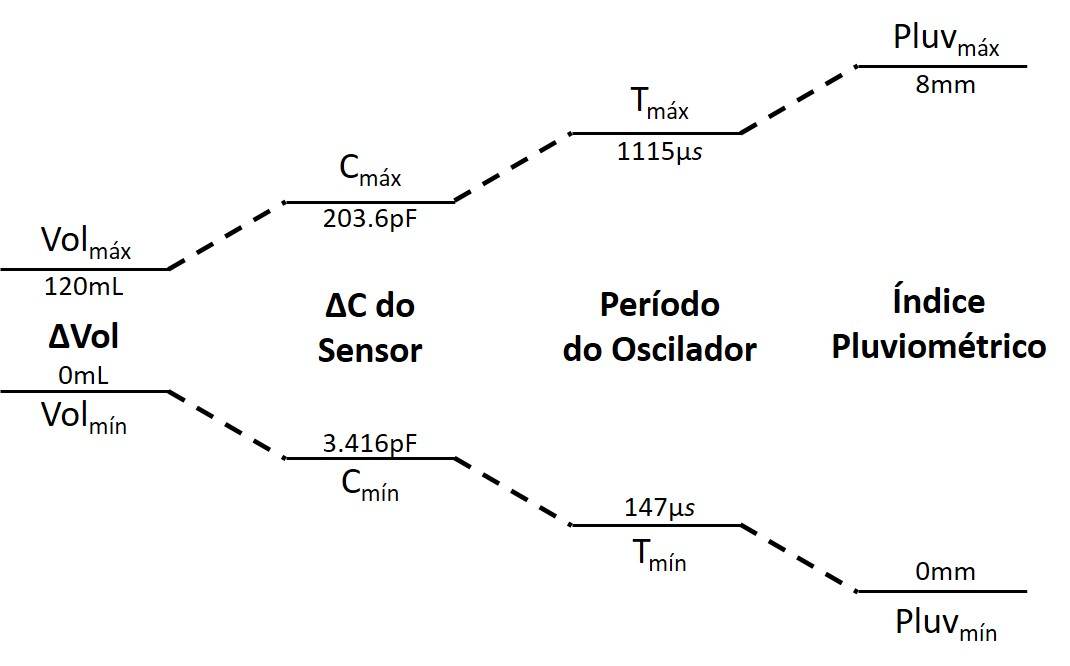
\includegraphics[width=\textwidth]{pluviometro-cadeia-medidas-proposta.jpg}
	\caption{Cadeia de medidas proposta para o pluviômetro a ser implementado.}
	\label{fig:pluviometro-cadeia-medidas-proposta}
\end{figure}

\chapter{Resultados e discussões}

\section{Termômetro}

Com base nas especificações do sensor Pt100 já estabelecidas, efetuou-se uma verificação do seu funcionamento, analisando-se a variação da sua resistência elétrica em função da variação de temperatura. O experimento realizado retornou os resultados que podem ser observados na Tabela \ref{tab:pt100-resistencia-exp}. Os valores foram verificados utilizando um multímetro Minipa modelo ET-2082 \cite{multimetro-minipa}, na faixa de 200$\Omega$, que apresenta precisão de $\pm 0.8\%$

\begin{table}[H]
\centering
\caption{Valores experimentais da variação da resistência elétrica do sensor Pt100 em função da variação da temperatura}
\label{tab:pt100-resistencia-exp}
\begin{tabular}{|c|c|c|}
\hline
\textbf{T(ºC)} & \textbf{R\_med($\Omega$)} & \textbf{Incerteza ($\Omega$)} \\ \hline
11.3           & 104.4                 & $\pm$ 0.8352                    \\ \hline
13.3           & 105.3                 & $\pm$ 0.8424                    \\ \hline
15.8           & 106.2                 & $\pm$ 0.8496                    \\ \hline
18.5           & 107.3                 & $\pm$ 0.8584                    \\ \hline
20.9           & 108.2                 & $\pm$ 0.8656                    \\ \hline
23.4           & 109.2                 & $\pm$ 0.8736                    \\ \hline
25.9           & 110.1                 & $\pm$ 0.8808                    \\ \hline
27.7           & 110.8                 & $\pm$ 0.8864                    \\ \hline
29.7           & 111.5                 & $\pm$ 0.8920                    \\ \hline
31.6           & 112.2                 & $\pm$ 0.8976                    \\ \hline
33.8           & 113.2                 & $\pm$ 0.9056                    \\ \hline
35.6           & 113.8                 & $\pm$ 0.9104                    \\ \hline
38.7           & 115.0                 & $\pm$ 0.9200                    \\ \hline
41.1           & 115.8                 & $\pm$ 0.9264                    \\ \hline
42.7           & 116.4                 & $\pm$ 0.9312                    \\ \hline
45.2           & 117.2                 & $\pm$ 0.9376                    \\ \hline
49.3           & 118.9                 & $\pm$ 0.9512                    \\ \hline
50.3           & 119.4                 & $\pm$ 0.9552                    \\ \hline
\end{tabular}
\end{table}


Na Figura \ref{fig:pt100-tf-experimental} é possível verificar o gráfico com os valores adquiridos e apresentados na Tabela \ref{tab:pt100-resistencia-exp} (pontos), bem como o traçado da função de transferência levantada por regressão linear (linha contínua), com base nos dados obtidos experimentalmente.

\begin{figure}[H]
	\centering 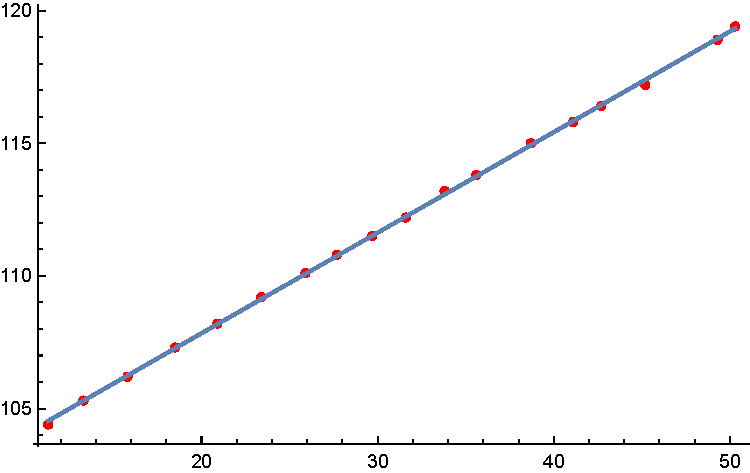
\includegraphics[width=\textwidth]{Temperatura/ResistenceTransferFunction.pdf}
	\caption{Amostra dos valores de resistência obtidos pela variação da temperatura do Pt100 e função de transferência experimental.}
	\label{fig:pt100-tf-experimental}
\end{figure}

A Equação \ref{eq:pt100-tf-experimental} apresenta a função de transferência experimental, levantada com base na regressão linear utilizando-se os valores constatados experimentalmente.

\begin{equation}
	R(T)=100.25+0.3792T
	\label{eq:pt100-tf-experimental}
\end{equation}

Apresentando um valor de $R^2$ de:

\begin{equation}
	R^2=0.9997
	\label{eq:pt100-r2-tf-experimental}
\end{equation}

Com base na função de transferência experimental apresentada na Equação \ref{eq:pt100-tf-experimental} é possível encontrar a sensibilidade experimental $S_{exp}$ do sistema, bem como o coeficiente de temperatura experimental $\alpha_{exp}$ do Pt100 utilizado.

\begin{equation}
	S_{exp}=\frac{dR(T)}{dT}=0.3792\frac{\Omega}{ºC}
	\label{eq:pt100-sensibilidade-experimental}
\end{equation}

\begin{equation}
	\alpha_{exp}=0.003783\Omega/\OmegaºC
	\label{eq:pt100-alpha-experimental}
\end{equation}

A Tabela \ref{tab:pt100-exp-teorico-tf-erro} faz um comparativo com os valores amostrados experimentalmente (Tabela \ref{tab:pt100-resistencia-exp}), os valores mediante utilização da função de transferência teórica (Equação \ref{eq:pt100-eq-teorica-valor}) e os valores com a utilização da função de transferência experimental (Equação \ref{eq:pt100-tf-experimental}). Apresenta também uma coluna com o cálculo do Erro de Linearidade experimental, na qual verifica-se o seu valor máximo de:

\begin{equation}
	\varepsilon_{L_{exp\%}}=0.15\%
	\label{eq:pt100-erro-linearidade-experimental}
\end{equation}

\begin{table}[H]
\centering
\caption{Valores experimentais, teóricos e pela função de transferência experimental regredida de $R(T)$ e o erro de linearidade observado.}
\label{tab:pt100-exp-teorico-tf-erro}
\begin{tabular}{|c|c|c|c|c|}
\hline
\textbf{$T(ºC)$} & \textbf{$R(T)_{exp}(\Omega)$} & \textbf{$R(T)_{teor}(\Omega)$} & \textbf{$R(T)_{ft}(\Omega)$} & \textbf{$\varepsilon_{L_{exp}}(\%)$} \\ \hline
11.3           & 104.4                 & 104.35                     & 104.53                & -0.15                        \\ \hline
13.3           & 105.3                 & 105.12                     & 105.29                & -0.14                        \\ \hline
15.8           & 106.2                 & 106.08                     & 106.24                & -0.13                        \\ \hline
18.5           & 107.3                 & 107.12                     & 107.27                & -0.12                        \\ \hline
20.9           & 108.2                 & 108.05                     & 108.18                & -0.11                        \\ \hline
23.4           & 109.2                 & 109.01                     & 109.12                & -0.10                        \\ \hline
25.9           & 110.1                 & 109.97                     & 110.07                & -0.08                        \\ \hline
27.7           & 110.8                 & 110.66                     & 110.75                & -0.07                        \\ \hline
29.7           & 111.5                 & 111.43                     & 111.51                & -0.07                        \\ \hline
31.6           & 112.2                 & 112.17                     & 112.23                & -0.06                        \\ \hline
33.8           & 113.2                 & 113.01                     & 113.07                & -0.05                        \\ \hline
35.6           & 113.8                 & 113.71                     & 113.75                & -0.04                        \\ \hline
38.7           & 115.0                 & 114.90                     & 114.93                & -0.02                        \\ \hline
41.1           & 115.8                 & 115.82                     & 115.84                & -0.01                        \\ \hline
42.7           & 116.4                 & 116.44                     & 116.44                & 0.00                         \\ \hline
45.2           & 117.2                 & 117.40                     & 117.39                & 0.01                         \\ \hline
49.3           & 118.9                 & 118.98                     & 118.94                & 0.03                         \\ \hline
50.3           & 119.4                 & 119.37                     & 119.32                & 0.03                         \\ \hline
\end{tabular}
\end{table}

Com o circuito condicionador montado em placa de circuito impresso, foram verificados os valores de saída do circuito, com o auxílio de uma década resistiva que simulou o funcionamento do sensor Pt100, aplicando os valores de resistência elétrica a partir da função de transferência experimental (Equação \ref{eq:pt100-tf-experimental} para os mesmos valores de temperaturas apresentados na primeira coluna da Tabela \ref{tab:pt100-exp-teorico-tf-erro}. Os resultados são observados na Tabela \ref{tab:termometro-simulacao-decada}.

\begin{table}[H]
\centering
\caption{Valores experimentais da tensão de saída do circuito de condicionamento, com o uso de década resistiva.}
\label{tab:termometro-simulacao-decada}
\begin{tabular}{|c|c|c|}
\hline
\textbf{T($ºC$)} & \textbf{$R_{Decada}(\Omega)$} & \textbf{Tensão Saída ($V$)} \\ \hline
11.3           & 104.5                    & -0.501                    \\ \hline
13.3           & 105.3                    & -0.372                    \\ \hline
15.8           & 106.2                    & -0.246                    \\ \hline
18.5           & 107.3                    & -0.088                    \\ \hline
20.9           & 108.2                    & 0.039                     \\ \hline
23.4           & 109.1                    & 0.177                     \\ \hline
25.9           & 110.1                    & 0.295                     \\ \hline
27.7           & 110.8                    & 0.397                     \\ \hline
29.7           & 111.5                    & 0.496                     \\ \hline
31.6           & 112.2                    & 0.581                     \\ \hline
33.8           & 113.1                    & 0.713                     \\ \hline
35.6           & 113.7                    & 0.794                     \\ \hline
38.7           & 114.9                    & 0.944                     \\ \hline
41.1           & 115.8                    & 1.054                     \\ \hline
42.7           & 116.4                    & 1.120                     \\ \hline
45.2           & 117.4                    & 1.217                     \\ \hline
49.3           & 118.9                    & 1.430                     \\ \hline
50.3           & 119.3                    & 1.490                     \\ \hline
\end{tabular}
\end{table}

Com base nos dados da Tabela \ref{tab:termometro-simulacao-decada}, pode-se efetuar uma regressão linear e obter a função de transferência experimental do circuito condicionado, com o uso da década resistiva simulando o sensor Pt100.

\begin{equation}
	V(T)=0.0503*T-1.0216
	\label{eq:termometro-tf-experimental-decada}
\end{equation}

Apresentando um valor de $R^2$ de:

\begin{equation}
	R^2=0.9985
	\label{eq:termometro-r2-tf-experimental-decada}
\end{equation}

E uma sensibilidade de:

\begin{equation}
	S_{exp}=50.3\frac{mV}{ºC}
	\label{eq:termometro-sensibilidade-experimental-decada}
\end{equation}

Comparando-se as equações de função de transferência teórica, com esta experimental simulada com a década, observa-se um erro de linearidade de 7.5$\%$. Porém, parte desse valor deve-se ao ajuste de zero diferenciado na simulação e no circuito real.

Por fim, foi realizado experimento com o circuito condicionador e o Pt100, cujo valores são apresentados na Tabela \ref{tab:termometro-experimento-pt100}.

\begin{table}[H]
\centering
\caption{Valores experimentais da tensão de saída da ponte e do circuito de condicionamento, com o uso do sensor Pt100.}
\label{tab:termometro-experimento-pt100}
\begin{tabular}{|c|c|c|}
\hline
\textbf{T($ºC$)} & \textbf{Tensão Ponte ($mV$)} & \textbf{Tensão Saída ($V$)} \\ \hline
5.6            & -0.9                      & -0.727                    \\ \hline
5.8            & -0.9                      & -0.702                    \\ \hline
6.9            & -0.8                      & -0.67                     \\ \hline
12.5           & -0.5                      & -0.408                    \\ \hline
14             & -0.4                      & -0.331                    \\ \hline
17.2           & -0.2                      & -0.165                    \\ \hline
19.3           & -0.1                      & -0.052                    \\ \hline
21.5           & 0.1                       & 0.059                     \\ \hline
23.5           & 0.2                       & 0.162                     \\ \hline
25.2           & 0.3                       & 0.259                     \\ \hline
26.7           & 0.4                       & 0.335                     \\ \hline
28.3           & 0.5                       & 0.422                     \\ \hline
30.8           & 0.7                       & 0.542                     \\ \hline
32.6           & 0.8                       & 0.628                     \\ \hline
34.2           & 0.9                       & 0.709                     \\ \hline
35.4           & 1.0                       & 0.765                     \\ \hline
38             & 1.1                       & 0.888                     \\ \hline
39.8           & 1.2                       & 0.978                     \\ \hline
42.1           & 1.4                       & 1.093                     \\ \hline
44.2           & 1.5                       & 1.202                     \\ \hline
47.1           & 1.6                       & 1.287                     \\ \hline
48.9           & 1.7                       & 1.38                      \\ \hline
50.3           & 1.9                       & 1.506                     \\ \hline
\end{tabular}
\end{table}

Com base na Tabela \ref{tab:termometro-experimento-pt100}, pode-se realizar uma regressão linear e obter-se a função de transferência final do sistema, tendo como base a temperatura, em $ºC$ e como saída a tensão, em $V$, conforme verifica-se na Equação \ref{eq:termometro-tf-experimental-pt100}.

\begin{equation}
	V(T)=0.0496*T-1.0043
	\label{eq:termometro-tf-experimental-pt100}
\end{equation}

Apresentando um valor de $R^2$ de:

\begin{equation}
	R^2=0.9993
	\label{eq:termometro-r2-tf-experimental-pt100}
\end{equation}

E uma sensibilidade de:

\begin{equation}
	S_{exp}=49.6\frac{mV}{ºC}
	\label{eq:termometro-sensibilidade-experimental-pt100}
\end{equation}

Comparando-se os valores obtidos por meio da função de transferência teórica geral com os valores obtidos para a função de transferência experimental geral, observa-se um erro de linearidade de 9.9$\%$, porém grande parte desse erro observado vem da diferença de ajuste de zero entre o circuito simulado e o circuito real.

A proposta inicial era fornecer um instrumento com um range de -10$ºC$ a +50$ºC$. Porém, nos experimentos realizados, não foi possível chegar a valores de temperatura tão baixos, sendo que a temperatura mais baixa alcançada foi de +5.6$ºC$. Assim, achou-se mais prudente alterar o range de trabalho para +5.0$ºC$ a +50.0$ºC$. Na Figura \ref{fig:termometro-cadeia-medidas-experimental} é apresentada a cadeia de medidas experimental do termômetro implementado.

\begin{figure}[H]
	\centering 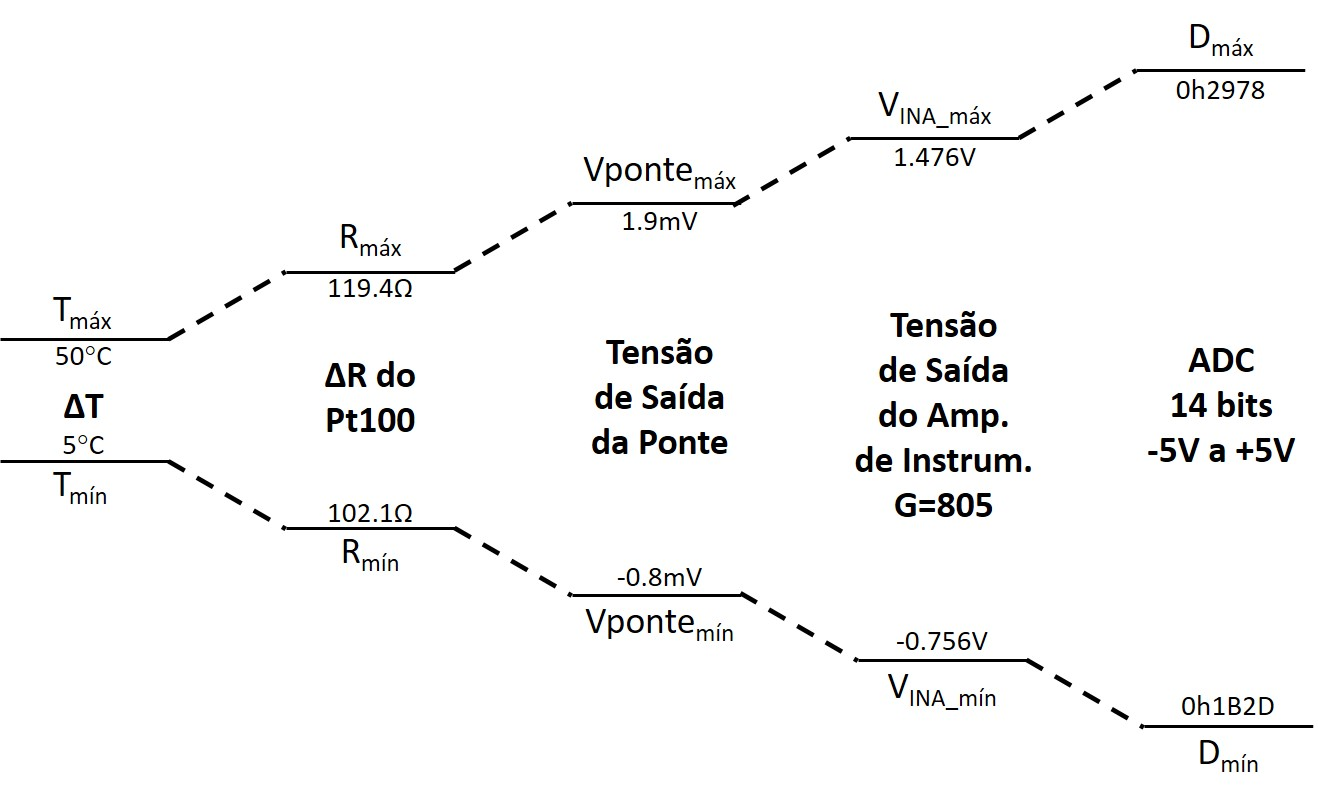
\includegraphics[width=\textwidth]{termometro-cadeia-medidas-experimental.jpg}
	\caption{Cadeia de Medidas experimental para o termômetro implementado.}
	\label{fig:termometro-cadeia-medidas-experimental}
\end{figure}

\todo{Resolução de entrada e de saída para cada etapa da cadeia de medidas}
\todo{análise de incerteza}

\section{Anemômetro}

Com base no circuito de condicionamento estipulado e na estrutura montada, com hastes de 18$cm$, foi aplicado vento centrado no copo de uma das hastes do anemômetro, fazendo o mesmo girar. O experimento foi realizado com duas intensidades de vento e três distâncias diferentes da boca do emissor do vento para o copo do anemômetro. As mesmas intensidades e distâncias foram aplicadas ao anemômetro digital comercial modelo LM-8010 \cite{anemometro-manual}, da Lutron Electronic. A Tabela \ref{tab:anemometro-amostras-comercial-periodo} apresenta os valores das intensidades e distâncias, o valor apresentado no anemômetro comercial e o período observado pela estrutura experimental, utilizando a interface criada no Labview.

\begin{table}[H]
\centering
\caption{Valores experimentais da velocidade do vento medido por anemômetro digital comercial e período de rotação do anemômetro experimental.}
\label{tab:anemometro-amostras-comercial-periodo}
\begin{tabular}{|c|c|c|c|}
\hline
\textbf{Intensidade} & \textbf{Distância ($cm$)} & \textbf{Vel comercial ($m/s$)} & \textbf{Período observado ($s$)} \\ \hline
med               & 60                      & 4.1$\pm$0.9                           & 0.720                          \\ \hline
max               & 60                      & 4.5$\pm$0.9                           & 0.591                          \\ \hline
med               & 40                      & 5.7$\pm$0.9                           & 0.535                          \\ \hline
med               & 20                      & 6.9$\pm$0.9                           & 0.476                          \\ \hline
max               & 40                      & 7.3$\pm$0.9                           & 0.412                          \\ \hline
max               & 20                      & 10.1$\pm$0.9                          & 0.327                          \\ \hline
\end{tabular}
\end{table}

Com os valores obtidos, pôde-se gerar uma função de transferência relacionando o período observado e os valores medidos experimentalmente com o anemômetro comercial, apresentada na Equação \ref{eq:anemometro-tf-experimental}.

\begin{equation}
	v(T)=15.0118-16.8067*T
	\label{eq:anemometro-tf-experimental}
\end{equation}

Apresentando um valor de $R^2$ de:

\begin{equation}
	R^2=0.8953
	\label{eq:anemometro-r2-tf-experimental}
\end{equation}

E uma sensibilidade de:

\begin{equation}
	S_{exp}=-16.8067\frac{m/s}{s}
	\label{eq:anemometro-sensibilidade-experimental}
\end{equation}

A Tabela \ref{tab:anemometro-comparativo-vtf-vtan} faz a comparação dos valores obtidos por meio da função de transferência experimental (Equação \ref{eq:anemometro-tf-experimental}) com o valor calculado da velocidade tangencial das extremidades das hastes da estrutura experimental, utilizando a Equação \ref{eq:anemometro-FT-proposta}.

\begin{table}[H]
\centering
\caption{Comparativo dos valores observados pelo anemômetro comercial, período de oscilação do anemômetro experimental, velocidade do vento por meio da função de tranferência experimental, velocidade tangencial experimental calculada e relação velocidade do vento pela função de transferência e velocidade tangencial.}
\label{tab:anemometro-comparativo-vtf-vtan}
\begin{tabular}{|c|c|c|c|c|}
\hline
\textbf{Vel comercial ($m/s$)} & \textbf{Período observado ($s$)} & \textbf{Vel FT ($m/s$)} & \textbf{V tan ($m/s$)} & \textbf{Rel (V FT/V tan)} \\ \hline
4.1                           & 0.720                          & 2.911                  & 1.570833333           & 54.0\%                      \\ \hline
4.5                           & 0.591                          & 5.079                  & 1.913705584           & 37.7\%                      \\ \hline
5.7                           & 0.535                          & 6.020                  & 2.114018692           & 35.1\%                      \\ \hline
6.9                           & 0.476                          & 7.012                  & 2.37605042            & 33.9\%                      \\ \hline
7.3                           & 0.412                          & 8.087                  & 2.745145631           & 33.9\%                      \\ \hline
10.1                          & 0.327                          & 9.516                  & 3.458715596           & 36.3\%                      \\ \hline
\end{tabular}
\end{table}

Com exceção da primeira medida, que está mais discrepante, os outros valores da relação da velocidade do vento pela função de transferência experimental com a velocidade tangencial experimental calculada, foram muito próximos um dos outros, o que leva a acreditar que o arrasto que a estrutura experimental insere no sistema é uma constante.

Em virtude das grandes incertezas quando da verificação das velocidades constatadas tanto pelo anemômetro comercial, quanto pelo anemômetro experimental, tendo em vista a dificuldade de se simular a ocorrência de vento, a menos que se utilize de um tunel de vento, o sistema apresenta um erro de linearidade um tanto alto, chegando a 11.8$\%$.

A Figura \ref{fig:anemometro-cadeia-medidas-experimental} apresenta a cadeia de medidas experimental levantada com base nos valores experimentais adquiridos e suas funções de tranferência experimentais.

\begin{figure}[H]
	\centering 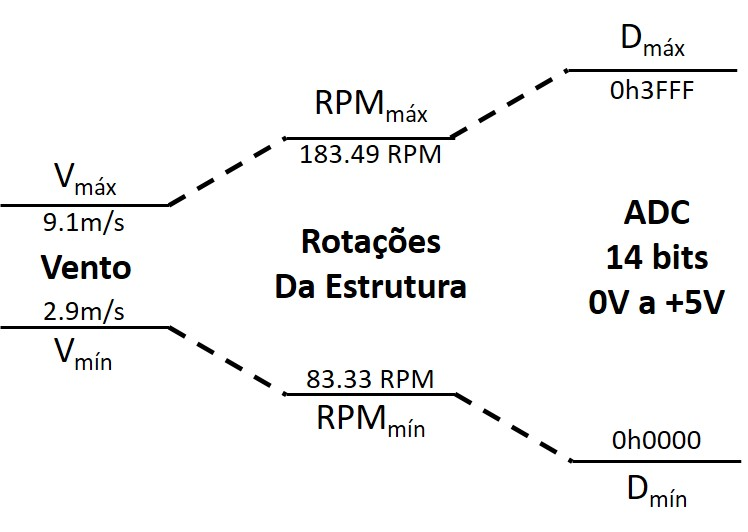
\includegraphics[width=0.5\textwidth]{anemometro-cadeia-medidas-experimental.jpg}
	\caption{Cadeia de Medidas experimental para o anemômetro implementado.}
	\label{fig:anemometro-cadeia-medidas-experimental}
\end{figure}


\section{Pluviômetro}
\subsection{Função de Transferência para a capacitância}

Todos os cálculos desta seção foram realizados no software Wolfram Mathematica versão 10.3.0 desenvolvido pela Wolfram Research, Inc. Os códigos utilizados estão em anexo no Anexo \todo{adicionar o anexo}.

A Tabela \ref{tab:resultados-pluviometro-capacitancia} apresenta os dados experimentais

\begin{longtable}{cc}
\caption{Valores de capacitância obtidos experimentalmente} \label{tab:resultados-pluviometro-capacitancia} \\
\textbf{$Volume (mL)$} & \textbf{$Capacitância (pF)$} \\ \hline
 0 & 89.5$\pm$ 0.895 \\
 1 & 86.1$\pm$ 0.861 \\
 2 & 72.5$\pm$ 0.725 \\
 3 & 84.9$\pm$ 0.849 \\
 4 & 49.$\pm$ 0.49 \\
 5 & 71$\pm$ 0.71 \\
 6 & 82.8$\pm$ 0.828 \\
 7 & 93.$\pm$ 0.93 \\
 8 & 87.$\pm$ 0.87 \\
 9 & 89.9$\pm$ 0.899 \\
 10 & 86.9$\pm$ 0.869 \\
 11 & 100.$\pm$ 1. \\
 12 & 85.$\pm$ 0.85 \\
 13 & 91.6$\pm$ 0.916 \\
 14 & 108.5$\pm$ 1.085 \\
 15 & 110.6$\pm$ 1.106 \\
 16 & 109.2$\pm$ 1.092 \\
 17 & 103.4$\pm$ 1.034 \\
 18 & 106.3$\pm$ 1.063 \\
 19 & 108.4$\pm$ 1.084 \\
 20 & 110.8$\pm$ 1.108 \\
 21 & 113.7$\pm$ 1.137 \\
 22 & 118.1$\pm$ 1.181 \\
 23 & 117.8$\pm$ 1.178 \\
 24 & 124.9$\pm$ 1.249 \\
 25 & 114.8$\pm$ 1.148 \\
 26 & 130.5$\pm$ 1.305 \\
 27 & 121.2$\pm$ 1.212 \\
 28 & 129.5$\pm$ 1.295 \\
 29 & 129.2$\pm$ 1.292 \\
 30 & 135.7$\pm$ 1.357 \\
 31 & 138.3$\pm$ 1.383 \\
 32 & 144.8$\pm$ 1.448 \\
 33 & 146.5$\pm$ 1.465 \\
 34 & 152.8$\pm$ 1.528 \\
 35 & 157.9$\pm$ 1.579 \\
 36 & 150.6$\pm$ 1.506 \\
 37 & 134.1$\pm$ 1.341 \\
 38 & 142.3$\pm$ 1.423 \\
 39 & 149.6$\pm$ 1.496 \\
 40 & 152.1$\pm$ 1.521 \\
 41 & 156.5$\pm$ 1.565 \\
 42 & 174.$\pm$ 1.74 \\
 43 & 166.$\pm$ 1.66 \\
 44 & 165.$\pm$ 1.65 \\
 45 & 164.4$\pm$ 1.644 \\
 46 & 158.6$\pm$ 1.586 \\
 47 & 154.5$\pm$ 1.545 \\
 48 & 144.9$\pm$ 1.449 \\
 49 & 172.8$\pm$ 1.728 \\
 50 & 181.$\pm$ 1.81 \\
 51 & 204.5$\pm$ 2.045 \\
 52 & 208.4$\pm$ 2.084 \\
 53 & 212.$\pm$ 2.12 \\
 54 & 213.2$\pm$ 2.132 \\
 55 & 216.8$\pm$ 2.168 \\
 56 & 221.9$\pm$ 2.219 \\
 57 & 225.8$\pm$ 2.258 \\
 58 & 228.4$\pm$ 2.284 \\
 59 & 231.4$\pm$ 2.314 \\
 60 & 233.4$\pm$ 2.334 \\
 61 & 237.2$\pm$ 2.372 \\
 62 & 238.6$\pm$ 2.386 \\
 63 & 241.7$\pm$ 2.417 \\
 64 & 243.7$\pm$ 2.437 \\
 65 & 247.3$\pm$ 2.473 \\
 66 & 250.4$\pm$ 2.504 \\
 67 & 254.5$\pm$ 2.545 \\
 68 & 256.1$\pm$ 2.561 \\
 69 & 258.2$\pm$ 2.582 \\
 70 & 179.3$\pm$ 1.793 \\
 71 & 215.1$\pm$ 2.151 \\
 72 & 252.4$\pm$ 2.524 \\
 73 & 255.2$\pm$ 2.552 \\
 74 & 263.1$\pm$ 2.631 \\
 75 & 266.6$\pm$ 2.666 \\
 76 & 268.$\pm$ 2.68 \\
 77 & 270.5$\pm$ 2.705 \\
 78 & 273.6$\pm$ 2.736 \\
 79 & 277.2$\pm$ 2.772 \\
 80 & 279.$\pm$ 2.79 \\
 81 & 281.1$\pm$ 2.811 \\
 82 & 285.3$\pm$ 2.853 \\
 83 & 286.6$\pm$ 2.866 \\
 84 & 291.1$\pm$ 2.911 \\
 85 & 293.4$\pm$ 2.934 \\
 86 & 294.9$\pm$ 2.949 \\
 87 & 295.7$\pm$ 2.957 \\
 88 & 297.4$\pm$ 2.974 \\
 89 & 303.6$\pm$ 3.036 \\
 90 & 313.9$\pm$ 3.139 \\
 91 & 312.9$\pm$ 3.129 \\
 92 & 314.2$\pm$ 3.142 \\
 93 & 317.7$\pm$ 3.177 \\
 94 & 322.7$\pm$ 3.227 \\
 95 & 324.3$\pm$ 3.243 \\
 96 & 327.2$\pm$ 3.272 \\
 97 & 329.5$\pm$ 3.295 \\
 98 & 332.7$\pm$ 3.327 \\
 99 & 335.7$\pm$ 3.357 \\
 100 & 335.4$\pm$ 3.354 \\
 101 & 336.1$\pm$ 3.361 \\
 102 & 340$\pm$ 3.4 \\
 103 & 341.3$\pm$ 3.413 \\
 104 & 345.6$\pm$ 3.456 \\
 105 & 346.2$\pm$ 3.462 \\
 106 & 350.2$\pm$ 3.502 \\
 107 & 353.1$\pm$ 3.531 \\
 108 & 355.3$\pm$ 3.553 \\
 109 & 358.1$\pm$ 3.581 \\
 110 & 359.6$\pm$ 3.596 \\
 111 & 363.9$\pm$ 3.639 \\
 112 & 367.6$\pm$ 3.676 \\
 113 & 369.7$\pm$ 3.697 \\
 114 & 372.9$\pm$ 3.729 \\
 115 & 376.4$\pm$ 3.764 \\
 116 & 377.5$\pm$ 3.775 \\
 117 & 378.8$\pm$ 3.788 \\
 118 & 384.7$\pm$ 3.847 \\
\end{longtable}

A Figura \ref{fig:tf:nivel:capacitancia} apresenta um gráfico com a função de transferência ajustada e os pontos medidos individualmente.

\begin{figure}[H]
	\centering 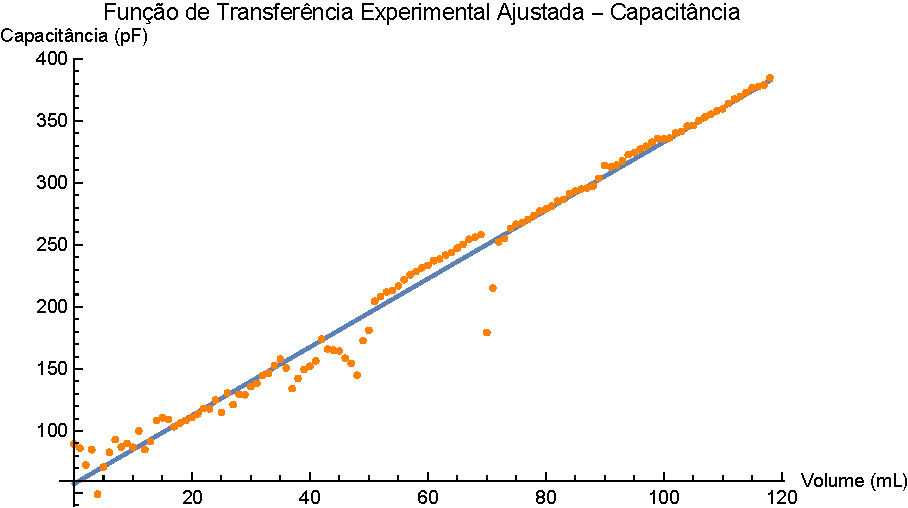
\includegraphics[width=\textwidth]{Nivel/Experimental/Capacitancia-Ajuste.pdf}
	\caption{Função de Transferência experimental da capacitância do sensor}
	\label{fig:tf:nivel:capacitancia}
\end{figure}

Na Figura \ref{fig:tf:nivel:capacitancia} a linha contínua é uma reta regredida por mínimos quadrados conforme Equação \ref{eq:tf:nivel:capacitancia}

\begin{equation}
	C(V) = 2.75376 V+57.3962
	\label{eq:tf:nivel:capacitancia}
\end{equation}
\noindent onde $C(V)$ é a capacitância do sensor dado um volume $V$ de água no recipiente.

A Equação \ref{eq:tf:nivel:capacitancia} foi ajustada com $R^2$ dado pela Equação \ref{eq:tf:nivel:capacitancia-r2} 

\begin{equation}
	R^2 = 0.99716
	\label{eq:tf:nivel:capacitancia-r2}
\end{equation}

A sensibilidade experimental para os valores de capacitância do sistema é dado pela Equação \ref{eq:resultados-pluviometro-capacitancia-sensibilidade}

\begin{equation}
	S = 2.75376 pF/mL
	\label{eq:resultados-pluviometro-capacitancia-sensibilidade}
\end{equation}

Pela Figura \ref{fig:tf:nivel:capacitancia} é possível aproximar o sensor como linear e obter erros inferiores a 5\%. Acredita-se que os pontos de discrepância das medidas ocorre devido ao erro do instrumento utilizado para estimar a capacitância.

Na Figura \ref{fig:resultados-pluviometro-capacitancia-comparacao} está apresentada uma comparação entre os valores de capacitância medidas e calculadas pela Equação \ref{eq:metodologia-pluviometro-capacitancia-teorico-final}.

\begin{figure}[H]
	\centering 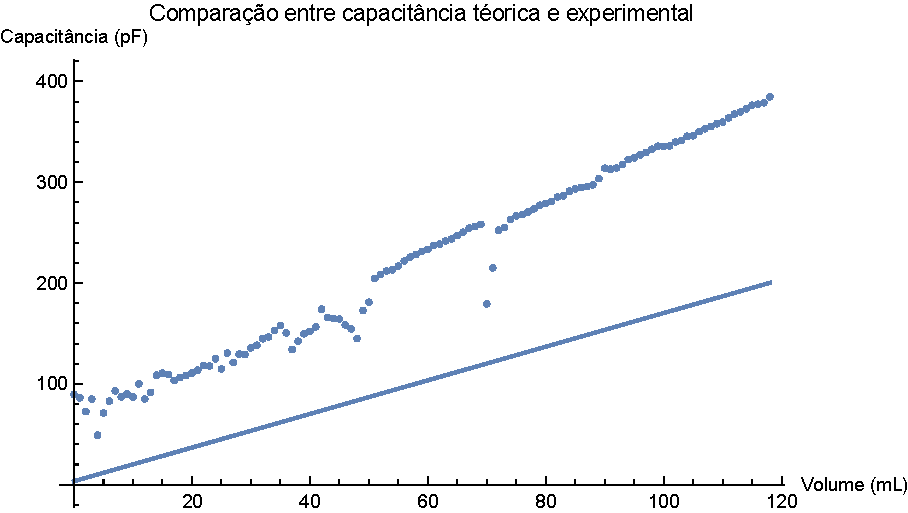
\includegraphics[width=\textwidth]{Nivel/Experimental/Capacitancia-Comparacao.pdf}
	\caption{Comparação entre a função de transferência experimental (pontos) e a função de transferência teórica (linha contínua).}
	\label{fig:resultados-pluviometro-capacitancia-comparacao}
\end{figure}

O erro de linearidade da medida de capacitância foi de 24.6\% devido ao fato de haver um deslocamento dos valores medidos e teóricos calculados decorrente da capacitância dos fios de conexão e imprecisão do instrumento que indicava erro de bateria fraca durante as medidas.

\subsection{Função de Transferência para a frequência do oscilador}

A Tabela \ref{tab:resultados-pluviometro-frequencia} apresenta as medidas experimentais individuais para a frequência de oscilação do oscilador para os volumes de líquido de 0 mL até 118 mL.

\begin{longtable}{cc}
\caption{Valores de frequência obtidos experimentalmente} \label{tab:resultados-pluviometro-frequencia} \\
\textbf{$Volume (mL)$} & \textbf{$Frequência (Hz) - 51ppm$} \\ \hline
 0 & 400 $\pm$ 0.020 \\
 1 & 500 $\pm$ 0.025 \\
 2 & 450 $\pm$ 0.023 \\
 3 & 440 $\pm$ 0.022 \\
 4 & 430 $\pm$ 0.022 \\
 5 & 480 $\pm$ 0.025 \\
 6 & 430 $\pm$ 0.022 \\
 7 & 430 $\pm$ 0.022 \\
 8 & 370 $\pm$ 0.019 \\
 9 & 370 $\pm$ 0.019 \\
 10 & 360 $\pm$ 0.019 \\
 11 & 360 $\pm$ 0.018 \\
 12 & 360 $\pm$ 0.018 \\
 13 & 350 $\pm$ 0.018 \\
 14 & 350 $\pm$ 0.018 \\
 15 & 340 $\pm$ 0.017 \\
 16 & 340 $\pm$ 0.017 \\
 17 & 330 $\pm$ 0.017 \\
 18 & 330 $\pm$ 0.017 \\
 19 & 320 $\pm$ 0.017 \\
 20 & 220 $\pm$ 0.011 \\
 21 & 370 $\pm$ 0.019 \\
 22 & 370 $\pm$ 0.019 \\
 23 & 370 $\pm$ 0.019 \\
 24 & 360 $\pm$ 0.019 \\
 25 & 360 $\pm$ 0.018 \\
 26 & 350 $\pm$ 0.018 \\
 27 & 350 $\pm$ 0.018 \\
 28 & 340 $\pm$ 0.017 \\
 29 & 330 $\pm$ 0.017 \\
 30 & 340 $\pm$ 0.017 \\
 31 & 330 $\pm$ 0.017 \\
 32 & 330 $\pm$ 0.017 \\
 33 & 320 $\pm$ 0.017 \\
 34 & 320 $\pm$ 0.016 \\
 35 & 320 $\pm$ 0.016 \\
 36 & 320 $\pm$ 0.016 \\
 37 & 310 $\pm$ 0.016 \\
 38 & 310 $\pm$ 0.016 \\
 39 & 310 $\pm$ 0.016 \\
 40 & 310 $\pm$ 0.016 \\
 41 & 310 $\pm$ 0.016 \\
 42 & 310 $\pm$ 0.016 \\
 43 & 300 $\pm$ 0.015 \\
 44 & 300 $\pm$ 0.015 \\
 45 & 300 $\pm$ 0.015 \\
 46 & 290 $\pm$ 0.015 \\
 47 & 290 $\pm$ 0.015 \\
 48 & 290 $\pm$ 0.015 \\
 49 & 290 $\pm$ 0.015 \\
 50 & 230 $\pm$ 0.012 \\
 51 & 230 $\pm$ 0.012 \\
 52 & 230 $\pm$ 0.012 \\
 53 & 230 $\pm$ 0.012 \\
 54 & 230 $\pm$ 0.012 \\
 55 & 230 $\pm$ 0.011 \\
 56 & 220 $\pm$ 0.011 \\
 57 & 220 $\pm$ 0.011 \\
 58 & 220 $\pm$ 0.011 \\
 59 & 210 $\pm$ 0.011 \\
 60 & 210 $\pm$ 0.011 \\
 61 & 210 $\pm$ 0.011 \\
 62 & 210 $\pm$ 0.011 \\
 63 & 210 $\pm$ 0.011 \\
 64 & 210 $\pm$ 0.011 \\
 65 & 210 $\pm$ 0.011 \\
 66 & 210 $\pm$ 0.011 \\
 67 & 210 $\pm$ 0.011 \\
 68 & 210 $\pm$ 0.011 \\
 69 & 210 $\pm$ 0.011 \\
 70 & 200 $\pm$ 0.010 \\
 71 & 240 $\pm$ 0.012 \\
 72 & 230 $\pm$ 0.012 \\
 73 & 230 $\pm$ 0.012 \\
 74 & 230 $\pm$ 0.012 \\
 75 & 230 $\pm$ 0.012 \\
 76 & 220 $\pm$ 0.011 \\
 77 & 220 $\pm$ 0.011 \\
 78 & 220 $\pm$ 0.011 \\
 79 & 210 $\pm$ 0.011 \\
 80 & 210 $\pm$ 0.011 \\
 81 & 210 $\pm$ 0.011 \\
 82 & 210 $\pm$ 0.011 \\
 83 & 210 $\pm$ 0.011 \\
 84 & 210 $\pm$ 0.011 \\
 85 & 210 $\pm$ 0.011 \\
 86 & 200 $\pm$ 0.010 \\
 87 & 200 $\pm$ 0.010 \\
 88 & 200 $\pm$ 0.010 \\
 89 & 200 $\pm$ 0.010 \\
 90 & 200 $\pm$ 0.010 \\
 91 & 200 $\pm$ 0.010 \\
 92 & 200 $\pm$ 0.0099 \\
 93 & 190 $\pm$ 0.0099 \\
 94 & 190 $\pm$ 0.0098 \\
 95 & 190 $\pm$ 0.0097 \\
 96 & 190 $\pm$ 0.0097 \\
 97 & 190 $\pm$ 0.0096 \\
 98 & 190 $\pm$ 0.0095 \\
 99 & 180 $\pm$ 0.0094 \\
 100 & 180 $\pm$ 0.0092 \\
 101 & 180 $\pm$ 0.0090 \\
 102 & 180 $\pm$ 0.0090 \\
 103 & 170 $\pm$ 0.0089 \\
 104 & 170 $\pm$ 0.0088 \\
 105 & 170 $\pm$ 0.0087 \\
 106 & 170 $\pm$ 0.0086 \\
 107 & 170 $\pm$ 0.0086 \\
 108 & 170 $\pm$ 0.0085 \\
 109 & 170 $\pm$ 0.0085 \\
 110 & 160 $\pm$ 0.0083 \\
 111 & 170 $\pm$ 0.0085 \\
 112 & 160 $\pm$ 0.0084 \\
 113 & 160 $\pm$ 0.0082 \\
 114 & 160 $\pm$ 0.0082 \\
 115 & 160 $\pm$ 0.0081 \\
 116 & 160 $\pm$ 0.0080 \\
 117 & 160 $\pm$ 0.0081 \\
 118 & 160 $\pm$ 0.0080 \\
\end{longtable}

A função de transferência da frequência de oscilação da onda quadrada do sistema de condicionamento é dada pela Figura \ref{fig:resultados-pluviometro-tf-frequencia}:

\begin{figure}[H]
	\centering 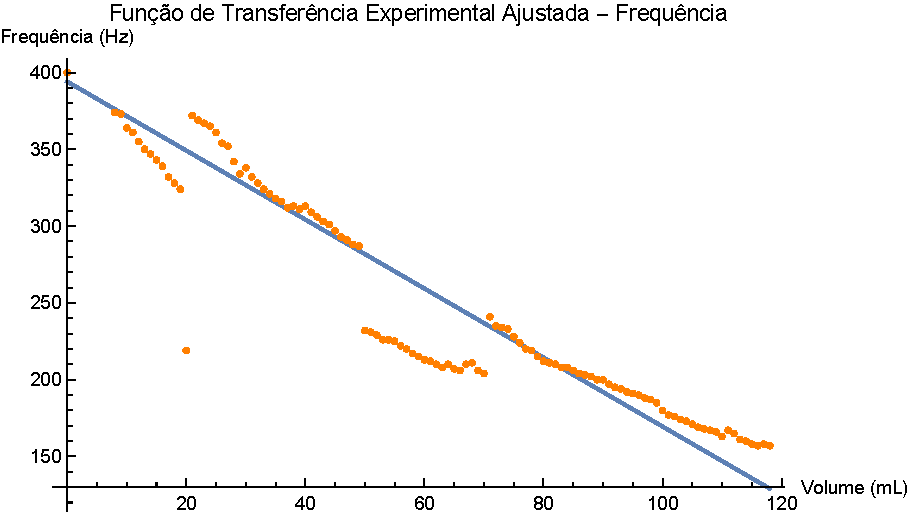
\includegraphics[width=\textwidth]{Nivel/Experimental/Frequencia-Ajuste.pdf}
	\caption{Função de Transferência experimental da frequência de oscilação do oscilador versus o volume de água contido no recipiente}
	\label{fig:resultados-pluviometro-tf-frequencia}
\end{figure}


Na Figura \ref{fig:resultados-pluviometro-tf-frequencia} a linha contínua é uma reta regredida por mínimos quadrados conforme Equação \ref{eq:resultados-pluviometro-tf-frequencia} e os pontos são as medidas experimentais obtidas em laboratório.

\begin{equation}
	f(V) = 394.095 - 2.24631 V
	\label{eq:resultados-pluviometro-tf-frequencia}
\end{equation}
\noindent onde $f(V)$ é a frequência de oscilação do oscilador com o sensor conectado e com volume $V$ de água no recipiente.

A Equação \ref{eq:resultados-pluviometro-tf-frequencia} foi ajustada com $R^2$ dado pela Equação \ref{eq:resultados-pluviometro-tf-frequencia-r2} 

\begin{equation}
	R^2 = 0.99716
	\label{eq:resultados-pluviometro-tf-frequencia-r2}
\end{equation}

A sensibilidade experimental para os valores de frequência do sistema é dado pela Equação \ref{eq:resultados-pluviometro-frequencia-sensibilidade}

\begin{equation}
	S = -2.24631 Hz/mL
	\label{eq:resultados-pluviometro-frequencia-sensibilidade}
\end{equation}

Na Figura \ref{fig:resultados-pluviometro-frequencia-comparacao} está apresentada uma comparação entre os valores de frequência medidas e calculadas.

\begin{figure}[H]
	\centering 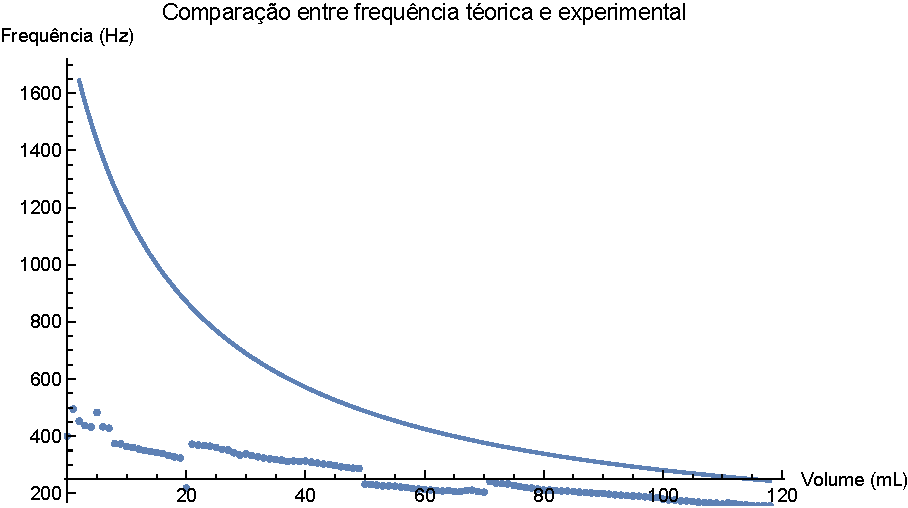
\includegraphics[width=\textwidth]{Nivel/Experimental/Frequencia-Comparacao.pdf}
	\caption{Comparação entre a função de transferência experimental (pontos) e a função de transferência teórica (linha contínua) da frequência de oscilação do oscilador.}
	\label{fig:resultados-pluviometro-frequencia-comparacao}
\end{figure}

O erro de conformidade da medida de frequência foi de 368\%. A confiança neste valor é baixa, o erro é amplificado pelo comportamento de $x^{-1}$ da curva, que magnifica os valores iniciais de frequência bem como a impedância de entrada pouco definida do amplificador operacional de entrada do circuito de condicionamento.

\subsection{Função de Transferência para a contagem de ciclos por oscilação}

A Tabela \ref{tab:resultados-pluviometro-ciclos} apresenta as medidas experimentais individuais para a contagem de ciclos por oscilação do oscilador para os volumes de líquido de 0 mL até 118 mL.

\begin{longtable}{cc}
\caption{Valores de frequência obtidos experimentalmente} \label{tab:resultados-pluviometro-ciclos} \\
\textbf{$Volume (mL)$} & \textbf{$Ciclos$} \\ \hline
 0 & 35132$\pm$ 1054 \\
 1 & 37486$\pm$ 1125 \\
 2 & 40850$\pm$ 1226 \\
 3 & 42334$\pm$ 1270 \\
 4 & 43008$\pm$ 1290 \\
 5 & 41820$\pm$ 1255 \\
 6 & 42070$\pm$ 1262 \\
 7 & 32801$\pm$ 984 \\
 8 & 43025$\pm$ 1291 \\
 9 & 43882$\pm$ 1316 \\
 10 & 44016$\pm$ 1320 \\
 11 & 44950$\pm$ 1349 \\
 12 & 45270$\pm$ 1358 \\
 13 & 45650$\pm$ 1370 \\
 14 & 46050$\pm$ 1382 \\
 15 & 46370$\pm$ 1391 \\
 16 & 46680$\pm$ 1400 \\
 17 & 47100$\pm$ 1413 \\
 18 & 48700$\pm$ 1461 \\
 19 & 49500$\pm$ 1485 \\
 20 & 49820$\pm$ 1495 \\
 21 & 49445$\pm$ 1483 \\
 22 & 49799$\pm$ 1494 \\
 23 & 49922$\pm$ 1498 \\
 24 & 50161$\pm$ 1505 \\
 25 & 50525$\pm$ 1516 \\
 26 & 50885$\pm$ 1527 \\
 27 & 51696$\pm$ 1551 \\
 28 & 53607$\pm$ 1608 \\
 29 & 54584$\pm$ 1638 \\
 30 & 54664$\pm$ 1640 \\
 31 & 54701$\pm$ 1641 \\
 32 & 55471$\pm$ 1664 \\
 33 & 56156$\pm$ 1685 \\
 34 & 56891$\pm$ 1707 \\
 35 & 57063$\pm$ 1712 \\
 36 & 57521$\pm$ 1726 \\
 37 & 58759$\pm$ 1763 \\
 38 & 58334$\pm$ 1750 \\
 39 & 58889$\pm$ 1767 \\
 40 & 58820$\pm$ 1765 \\
 41 & 59876$\pm$ 1796 \\
 42 & 60012$\pm$ 1800 \\
 43 & 60470$\pm$ 1814 \\
 44 & 61385$\pm$ 1842 \\
 45 & 62069$\pm$ 1862 \\
 46 & 62462$\pm$ 1874 \\
 47 & 62864$\pm$ 1886 \\
 48 & 63658$\pm$ 1910 \\
 49 & 64137$\pm$ 1924 \\
 50 & 65700$\pm$ 1971 \\
 51 & 66457$\pm$ 1994 \\
 52 & 66564$\pm$ 1997 \\
 53 & 66634$\pm$ 1999 \\
 54 & 69120$\pm$ 2074 \\
 55 & 69039$\pm$ 2071 \\
 56 & 68550$\pm$ 2057 \\
 57 & 69683$\pm$ 2090 \\
 58 & 70506$\pm$ 2115 \\
 59 & 69606$\pm$ 2088 \\
 60 & 70856$\pm$ 2126 \\
 61 & 71955$\pm$ 2159 \\
 62 & 72584$\pm$ 2178 \\
 63 & 72565$\pm$ 2177 \\
 64 & 72764$\pm$ 2183 \\
 65 & 73350$\pm$ 2201 \\
 66 & 73667$\pm$ 2210 \\
 67 & 74037$\pm$ 2221 \\
 68 & 74546$\pm$ 2236 \\
 69 & 75906$\pm$ 2277 \\
 70 & 77431$\pm$ 2323 \\
 71 & 77081$\pm$ 2312 \\
 72 & 77095$\pm$ 2313 \\
 73 & 78513$\pm$ 2355 \\
 74 & 79193$\pm$ 2376 \\
 75 & 80757$\pm$ 2423 \\
 76 & 82842$\pm$ 2485 \\
 77 & 82744$\pm$ 2482 \\
 78 & 83908$\pm$ 2517 \\
 79 & 85830$\pm$ 2575 \\
 80 & 86328$\pm$ 2590 \\
 81 & 87064$\pm$ 2612 \\
 82 & 87765$\pm$ 2633 \\
 83 & 89036$\pm$ 2671 \\
 84 & 88383$\pm$ 2652 \\
 85 & 89184$\pm$ 2676 \\
 86 & 89963$\pm$ 2699 \\
 87 & 90343$\pm$ 2710 \\
 88 & 91270$\pm$ 2738 \\
 89 & 92768$\pm$ 2783 \\
 90 & 92808$\pm$ 2784 \\
 91 & 93586$\pm$ 2808 \\
 92 & 95212$\pm$ 2856 \\
 93 & 94823$\pm$ 2845 \\
 94 & 95428$\pm$ 2863 \\
 95 & 96383$\pm$ 2891 \\
 96 & 97512$\pm$ 2925 \\
 97 & 98066$\pm$ 2942 \\
 98 & 98428$\pm$ 2953 \\
 99 & 99034$\pm$ 2971 \\
 100 & 102584$\pm$ 3078 \\
 101 & 103142$\pm$ 3094 \\
 102 & 104111$\pm$ 3123 \\
 103 & 105461$\pm$ 3164 \\
 104 & 105806$\pm$ 3174 \\
 105 & 104868$\pm$ 3146 \\
 106 & 107401$\pm$ 3222 \\
 107 & 108077$\pm$ 3242 \\
 108 & 109047$\pm$ 3271 \\
 109 & 109381$\pm$ 3281 \\
 110 & 110243$\pm$ 3307 \\
 111 & 111285$\pm$ 3339 \\
 112 & 112573$\pm$ 3377 \\
 113 & 113507$\pm$ 3405 \\
 114 & 114288$\pm$ 3429 \\
 115 & 114869$\pm$ 3446 \\
 116 & 116016$\pm$ 3480 \\
 117 & 116015$\pm$ 3480 \\
 118 & 117082$\pm$ 3512 \\
\end{longtable}

A função de transferência da contagem de ciclos do processador para cada oscilação da onda quadrada do sistema de condicionamento é dada pela Figura \ref{fig:resultados-pluviometro-tf-ciclos}:

\begin{figure}[H]
	\centering 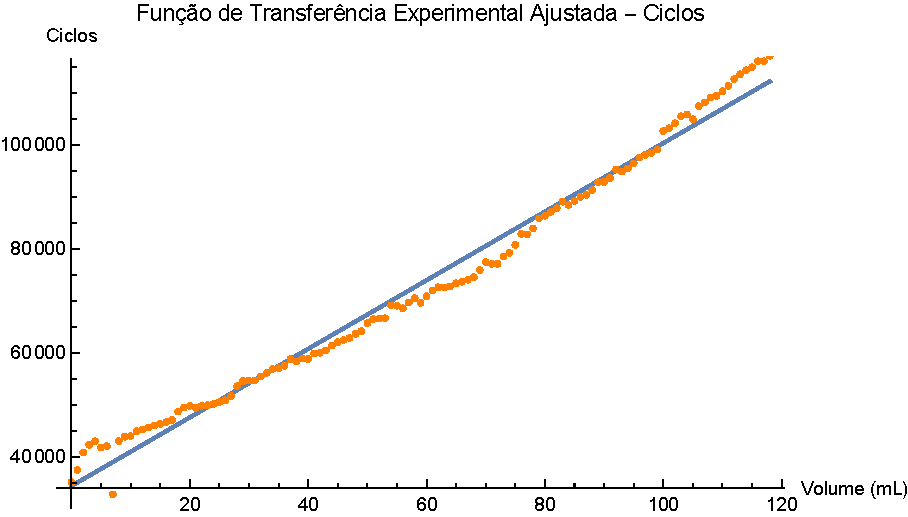
\includegraphics[width=\textwidth]{Nivel/Experimental/Ciclos-Ajuste.pdf}
	\caption{Função de Transferência experimental da contagem de ciclos do processador para cada oscilação da onda quadrada versus o volume de água contido no recipiente}
	\label{fig:resultados-pluviometro-tf-ciclos}
\end{figure}


Na Figura \ref{fig:resultados-pluviometro-tf-ciclos} a linha contínua é uma reta regredida por mínimos quadrados conforme Equação \ref{eq:resultados-pluviometro-tf-ciclos} e os pontos são as medidas experimentais obtidas em laboratório.

\begin{equation}
	n(V) = 34409.2 + 658.776 V
	\label{eq:resultados-pluviometro-tf-ciclos}
\end{equation}
\noindent onde $n(V)$ é o número de ciclos do processador em um período de oscilação do oscilador com o sensor conectado e com volume $V$ de água no recipiente.

A Equação \ref{eq:resultados-pluviometro-tf-ciclos} foi ajustada com $R^2$ dado pela Equação \ref{eq:resultados-pluviometro-tf-ciclos-r2} 

\begin{equation}
	R^2 = 0.998731
	\label{eq:resultados-pluviometro-tf-ciclos-r2}
\end{equation}

A sensibilidade experimental para o número de ciclos por oscilação do oscilador do sistema é dado pela Equação \ref{eq:resultados-pluviometro-ciclos-sensibilidade}

\begin{equation}
	S = 658.776 ciclos/mL
	\label{eq:resultados-pluviometro-ciclos-sensibilidade}
\end{equation}

Logo, conforme esperado pela Equação \ref{eq:metologia-pluviometro-periodo} apresentada na metodologia experimental, o comportamento do período de oscilação é linear em função da capacitância.

Na Figura \ref{fig:resultados-pluviometro-ciclos-comparacao} está apresentada uma comparação entre os números de ciclos contados em cada oscilação medida e calculada pela Equação \ref{eq:metodologia-pluviometro-ciclos-teorico}.

\begin{figure}[H]
	\centering 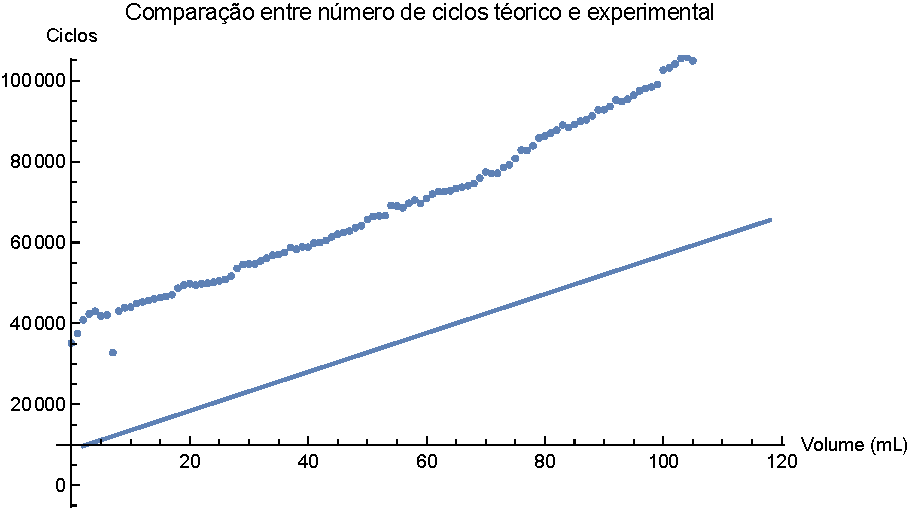
\includegraphics[width=\textwidth]{Nivel/Experimental/Ciclos-Comparacao.pdf}
	\caption{Comparação entre a função de transferência experimental (pontos) e a função de transferência teórica (linha contínua) para a contagem de ciclos por oscilação.}
	\label{fig:resultados-pluviometro-ciclos-comparacao}
\end{figure}

O erro de linearidade da medida de contagem de ciclos foi de 14.03\%.

\subsection{Função de Transferência para a equação de compensação}

A função de transferência da equação de compensação do sistema em função do volume de água dentro do recipiente do sensor está apresentada na Figura \ref{fig:resultados-pluviometro-tf-compensado}

\begin{figure}[H]
	\centering 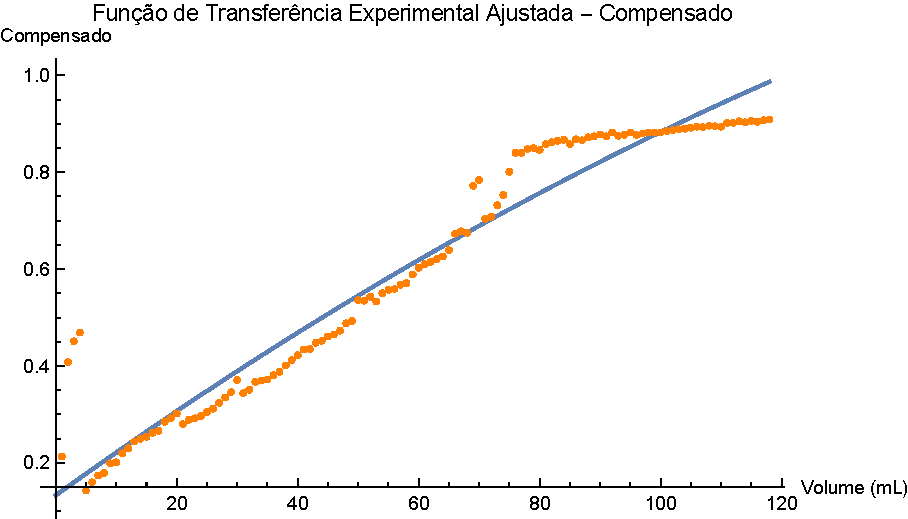
\includegraphics[width=\textwidth]{Nivel/Experimental/Compensado-Ajuste.pdf}
	\caption{Função de Transferência experimental da medida compensada de tempo em função da quantidade de volume dentro do recipiente do sensor.}
	\label{fig:resultados-pluviometro-tf-compensado}
\end{figure}


Na Figura \ref{fig:resultados-pluviometro-tf-compensado} a linha contínua é uma reta regredida por mínimos quadrados conforme Equação \ref{eq:resultados-pluviometro-tf-compensado} e os pontos são as medidas experimentais obtidas em laboratório.

\begin{equation}
	N(V) = 0.133032 + 0.00898593 V - 0.0000148452 V^2
	\label{eq:resultados-pluviometro-tf-compensado}
\end{equation}
\noindent onde $N(V)$ é a quantidade adimensional calculada após a compensação dos sensores pela equação \ref{eq:metodologia-pluviometro-compensacao} do sistema completo e com volume $V$ de água no recipiente.

A Equação \ref{eq:resultados-pluviometro-tf-compensado} foi ajustada com $R^2$ dado pela Equação \ref{eq:resultados-pluviometro-tf-compensado-r2} 

\begin{equation}
	R^2 = 0.989612
	\label{eq:resultados-pluviometro-tf-compensado-r2}
\end{equation}

A sensibilidade experimental para a equação de compensação do sistema é dado pela Equação \ref{eq:resultados-pluviometro-compensado-sensibilidade}

\begin{equation}
	S = 0.00898593 - 0.0000296905 \text{ mL}^{-1}
	\label{eq:resultados-pluviometro-compensado-sensibilidade}
\end{equation}

Devido aos sensores de compensação, em especial o sensor de referência de líquido, o sistema perdeu a característica linear. Isto se deve ao fato da referência não ser perfeitamente fixa durante a execução do experimento, isto é, a capacitância continuava variando a medida que água fosse adicionada ao recipiente. Este efeito pode ser compensado caso seja usada uma referência de líquido externa, semelhante à referência de ambiente.

Na Figura \ref{fig:resultados-pluviometro-compensacao-comparacao} está apresentada uma comparação entre o valor N do sistema medido e calculado pela Equação \ref{eq:metodologia-pluviometro-compensacao}.

\begin{figure}[H]
	\centering 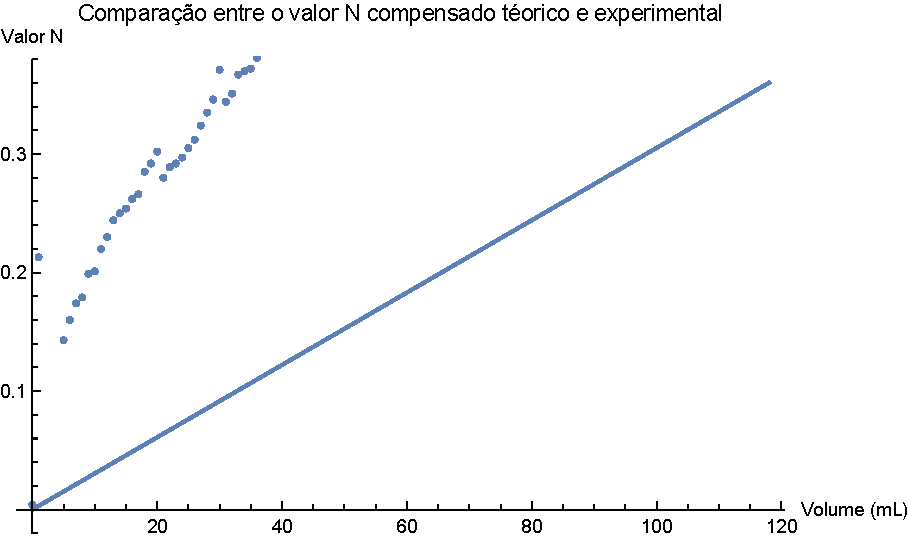
\includegraphics[width=\textwidth]{Nivel/Experimental/Compensado-Comparacao.pdf}
	\caption{Comparação entre a função de transferência experimental (pontos) e a função de transferência teórica (linha contínua) para a função de compensação.}
	\label{fig:resultados-pluviometro-compensacao-comparacao}
\end{figure}

O erro de linearidade da medida pela função de compensação foi de 66.86\%.

 Figura \ref{fig:pluviometro-cadeia-medidas-experimental} apresenta a cadeia de medidas experimental levantada com base nos valores experimentais adquiridos e suas funções de tranferência experimentais.

\begin{figure}[H]
	\centering 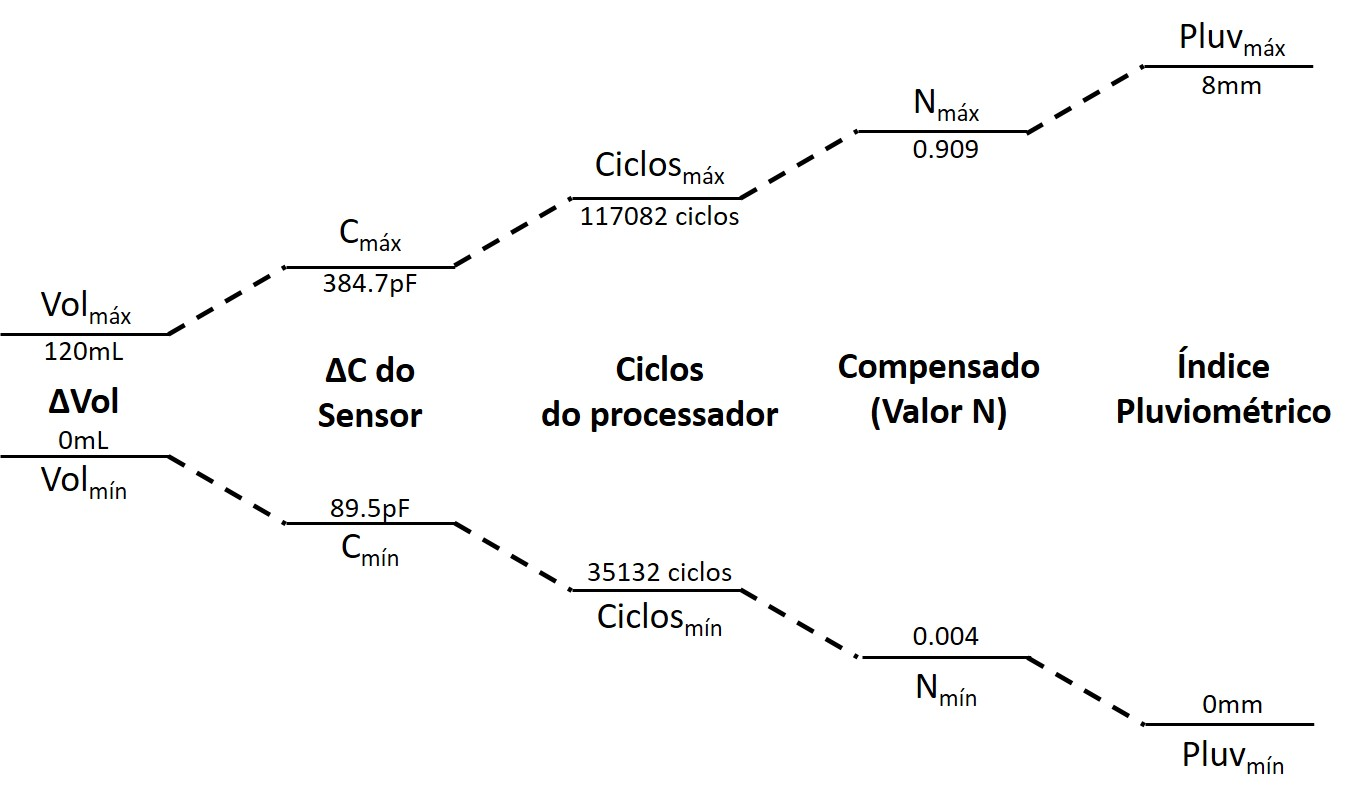
\includegraphics[width=0.8\textwidth]{pluviometro-cadeia-medidas-experimental.jpg}
	\caption{Cadeia de Medidas experimental para o pluviômetro implementado.}
	\label{fig:pluviometro-cadeia-medidas-experimental}
\end{figure}

\chapter{Conclusão}

O presente projeto se propôs à elaboração de uma central meteorológica experimental contendo termômetro, anemômetro e pluviômetro.

O termômetro foi construído utilizando um sensor termoresistivo Pt100, que apresenta uma boa linearidade dentro da faixa de aplicação do projeto. Inicialmente foi proposto um range de -10$ºC$ a +50$ºC$. Porém, por problema de simulação de temperaturas abaixo de 0$ºC$, optou-se por alterar o range para +5$ºC$ a +50$ºC$. O sensor foi montado em uma ponte de Wheatstone com ajuste de balanço e ajuste de zero para a saída do amplificador de instrumentação. A saída do amplificador de instrumentação foi conectada à DAQ NI USB-6009 a qual aplica a função de transferência experimental na tensão observada e retorna o valor da temperatura correspondente. O circuito apresentou erro de linearidade de 9.9$\%$ muito em virtude de diferenças nos ajustes de zero do circuito teórico e do circuito experimental.

Para o anemômetro foi utilizado um sensor de efeito Hall linear, porém, como a intenção de seu uso era exclusivamente a contagem de voltas, seu funcionamento foi condicionado a um circuito de chaveamento, que fica em nível alto até perceber a presença do ímã, quando então passa para nível baixo. Esse circuito então apresenta a sua saída como uma onda quadrada, na qual é possível fazer a contagem da duração do período de cada volta. Para obter valores comparativos a fim de se gerar a função de trasferência experimental, foi utilizado um anemômetro digital comercial submetido às mesmas condições que o anemômetro experimental. O resultado final apresentou um erro de linearidade de 11.8$\%$. Esse erro elevado deve-se ao fato de as simulações experimentais não terem sido executadas em ambientes controlados como, por exemplo, um tunel de vento.

O pluviômetro 

\newpage
\begin{thebibliography}{9}
\bibitem{mathematica-numerial-precision} \url{https://reference.wolfram.com/language/tutorial/NumericalPrecision.html}, acessado em 16 de março de 2016

\bibitem{livro-texto}  Balbinot, A.; Brusamarello, V. J., Instrumentação e Fundamentos de Medida - Vol.1 - 2ª Ed. Rio de Janeiro: LTC, 2014.

\bibitem{anemometro-manual} Manual do Anemômetro LM-8010, da Lutron Electronic, disponível em \url{http://eshop.micronix.cz/data/cz/att/002/4582-2595.pdf}.

\bibitem{capacitor-plano} Binns, K. J.; Lawrenson, P. J., Analysis and Computation of Electric and Magnetic Field Problems - 2ª Ed., Pergamon Press, 1973.

\bibitem{estacao} \url{https://pt.wikipedia.org/wiki/Esta\%C3\%A7\%C3\%A3o_meteorol\%C3\%B3gica}, acessado em 16/04/2016.

\bibitem{pluviometro} \url{https://pt.wikipedia.org/wiki/Pluvi\%C3\%B4metro}, acessado em 16/04/2016.

\bibitem{pluviometro-1} \url{http://www.agsolve.com.br/dicas-e-solucoes/como-funciona-o-pluviometro}, acessado em 16/04/2016.

\bibitem{datasheet-hall} Datasheet do sensor de efeito Hall SS94A2, da Honeywell, disponível em \url{http://docs-europe.electrocomponents.com/webdocs/0098/0900766b80098534.pdf}.

\bibitem{catalogo-pt100} Catálogo de sensores resistivos de platina da LABFACILITY, \url{http://www.farnell.com/datasheets/1848446.pdf }, acessado em 31/05/2016.

\bibitem{datasheet-INA126} Datasheet do amplificador de instrumentação INA126, da Texas Instruments, disponível em \url{http://www.ti.com.cn/cn/lit/ds/symlink/ina126.pdf}.

\bibitem{pluviometro-capacitivo-texas} Capacitive-Based Liquid Level Sensing Sensor Reference Design, \url{http://www.ti.com/lit/ug/tidu736a/tidu736a.pdf
}, acessado em 30/05/2016.

\bibitem{medicao-capacitancia} Use Analog Techniques To Measure Capacitance In Capacitive Sensors, \url{http://m.electronicdesign.com/analog/use-analog-techniques-measure-capacitance-capacitive-sensors}, acessado em 01/06/2016.

\bibitem{multimetro-minipa} Manual do multímetro digital Minipa ET-2082B, disponível em \url{http://portal.if.usp.br/labdid/sites/portal.if.usp.br.labdid/files/Et-2082b-1100.pdf}.

\bibitem{ponte-minipa} Manual da Ponte LCR Minipa MX-1010, disponível em \url{http://www.multcomercial.com.br/pdf/minipa/Mx-1010-1100.pdf}.


%\bibitem{ref1} Sobrenome, A.B.; Sobrenome, C.D. Title of the cited article. Journal Title 2007, 6, 100-110. 
%\bibitem{ref2} Balbinot, A.; Brusamarello, V.J.. Title of the cited article. Journal Title 2007, 6, 100-110. 
%\bibitem{ref3} Author, A.; Author, B. Title of the chapter. In Book Title, 2nd ed.; Editor, A., Editor, B., Eds.; Publisher: Publisher Location, Country, 2007; Volume 3, pp. 154-196.
%\bibitem{ref4} Author, A.; Author, B. Book Title, 3rd ed.; Publisher: Publisher Location, Country, 2008; 
%pp. 154-196.

\end{thebibliography}

\end{document}
